% !TEX TS-program = lualatex
% !TEX encoding = UTF-8 Unicode
% --- Preamble: Styling ---
\documentclass[a4paper,12pt]{article}
\usepackage[left=3cm,top=3cm,bottom=2cm,right=2cm]{geometry}

% Encoding & Language
\usepackage[utf8]{inputenc}
\usepackage[T1]{fontenc}
\usepackage[portuguese]{babel}
\addto\extrasportuguese{\renewcommand{\contentsname}{Índice}}

% Margins, Columns, Indentation & Spacing
\usepackage{multicol}
\usepackage{indentfirst}
\usepackage{ragged2e}  % For extendability
\usepackage{setspace}
\onehalfspacing
\setlength{\columnsep}{1cm}

% Headers, Titles, Footnotes & Captioning
\usepackage{sectsty}
\usepackage{titling}
\renewcommand\maketitlehooka{\null\mbox{}\vfill}
\renewcommand\maketitlehookd{\vfill\null}
\usepackage{footmisc}
\usepackage{caption}
\captionsetup[figure]{font=footnotesize}

% Graphics Support
\usepackage{graphicx}
\graphicspath{{./assets/}}
\usepackage{svg}
\usepackage{tikz}
\usepackage{float}
\usepackage{fancyhdr}
\usepackage{xcolor}
\usetikzlibrary{shapes,shadows,arrows,positioning,calc}
\tikzstyle{RectObject}=[rectangle,fill=white,draw,line width=0.5mm]
\tikzstyle{line}=[draw]
\tikzstyle{arrow}=[draw, -latex]

% --- Preamble: Commands ---
\pagestyle{fancy}
\fancyhf{}
\fancyfoot[R]{\thepage}
\renewcommand{\headrulewidth}{0pt}

% --- Document: Begin ---
\begin{document}
% --- Document: Title Page ---
\begin{titlingpage}
    \begin{center}
        {\large
            % Institution
            {\Huge
                FATEC -- Prof. Waldomiro May	
            }\\

			\vspace{1cm}
            ANÁLISE E DESENVOLVIMENTO DE SISTEMAS

            % Project Presentation
            \vspace{1cm}
            PROJETO INTEGRADOR I

            % Project Logo
            \vspace{6cm}
            \raisebox{-0.75em}{
\includegraphics[scale=0.1]{neotasker-logo.png}}
            % Project Name
            {\Huge
                \textbf{NeoTasker}
            }

            % Project Description
            Agenda Pessoal

            % Authors
            \vspace{2cm}
            CHRYSTIAN M. FRANKLIN \\
            WELLINGTON E. RODRIGUES

            % Date
            \vspace{8cm}
            2023.2
        }
    \end{center}
\end{titlingpage}

% --- Document: Table of Contents ---
\setcounter{tocdepth}{4}
\tableofcontents
\pagebreak

% --- Document: Table of Figures ---
\listoffigures
\pagebreak

% --- Document: Content ---
% --- Segment: Introduction ---
\section{Introdução}
\subsection{Tema}
O software \textbf{NeoTasker} é um \textit{Sistema de Gerenciamento de Agenda Pessoal}. Este caracteriza-se pelo controle de atividades 
e eventos decorrentes do dia-a-dia de um indivíduo.

\subsection{Justificativa de Escolha do Tema}
A organização pessoal é uma tarefa árdua e frequentemente mais complexa do que imaginada, especialmente quando é considerado as rotinas 
frenéticas de estudantes e trabalhadores, devido ao seu vasto e variado uso de tempo, com suas rotinas crescentemente mais corridas.

A partir dessa consideração, o tema de \textbf{agenda pessoal} foi selecionado devido à familiaridade do ambiente dos autores, em 
conjunto com as possibilidades de diferentes soluções relacionadas ao aspecto de controle de tempo e organização de rotinas.

\subsection{Descrição do Problema}
O sistema deve ser capaz de efetuar o agendamento, modificação, consultas e remoção dos diferentes tipos de atividades presentes 
de maneira individual. Além de apresentar relatórios e informações estatísticas sobre as atividades e o uso do sistema, visando 
melhorar a experiência do usuário em relação a sua organização de tempo.

\subsection{Objetivos do Projeto}
Este projeto é caracterizado por ser uma atividade conjunta com o objetivo de desenvolver os conteúdos das seguintes 
disciplinas do segundo período do curso de análise e desenvolvimento de sistemas:
\begin{itemize}
    \item \textbf{IES100:} Engenharia de Software I;
    \item \textbf{IHC001:} Interação Humano Computador;
    \item \textbf{ILP010:} Linguagem de Programação;
    \item \textbf{ISI002:} Sistemas de Informação.
\end{itemize}

Além do aspecto disciplinar, este projeto tem como objetivos secundários o desenvolvimento de habilidades essenciais no 
atual ambiente de trabalho:
\begin{itemize}
    \item A produção de um projeto relacionado ao \textbf{Gerenciamento de Tempo e Rotina};
    \item A execução da \textbf{Metodologia Ágil} e \textbf{SCRUM};
    \item A \textbf{Análise de Projetos} e o \textbf{Levantamento de Requisitos};
    \item A \textbf{Consideração de Aspectos de Acessibilidade};
    \item A \textbf{Produção de Documentação e Manuais};
    \item O \textbf{Desenvolvimento de Sistemas de Softwares Completos};
    \item A \textbf{Implementação de Caso de Testes}.
\end{itemize}

\subsection{Organização do Projeto}
\subsubsection{Estrutura do Projeto}
O projeto está estruturado a partir da organização de projetos em cascatas, com base na seguinte visão:

\vspace{1em}
\begin{figure}[H]
    \centering
    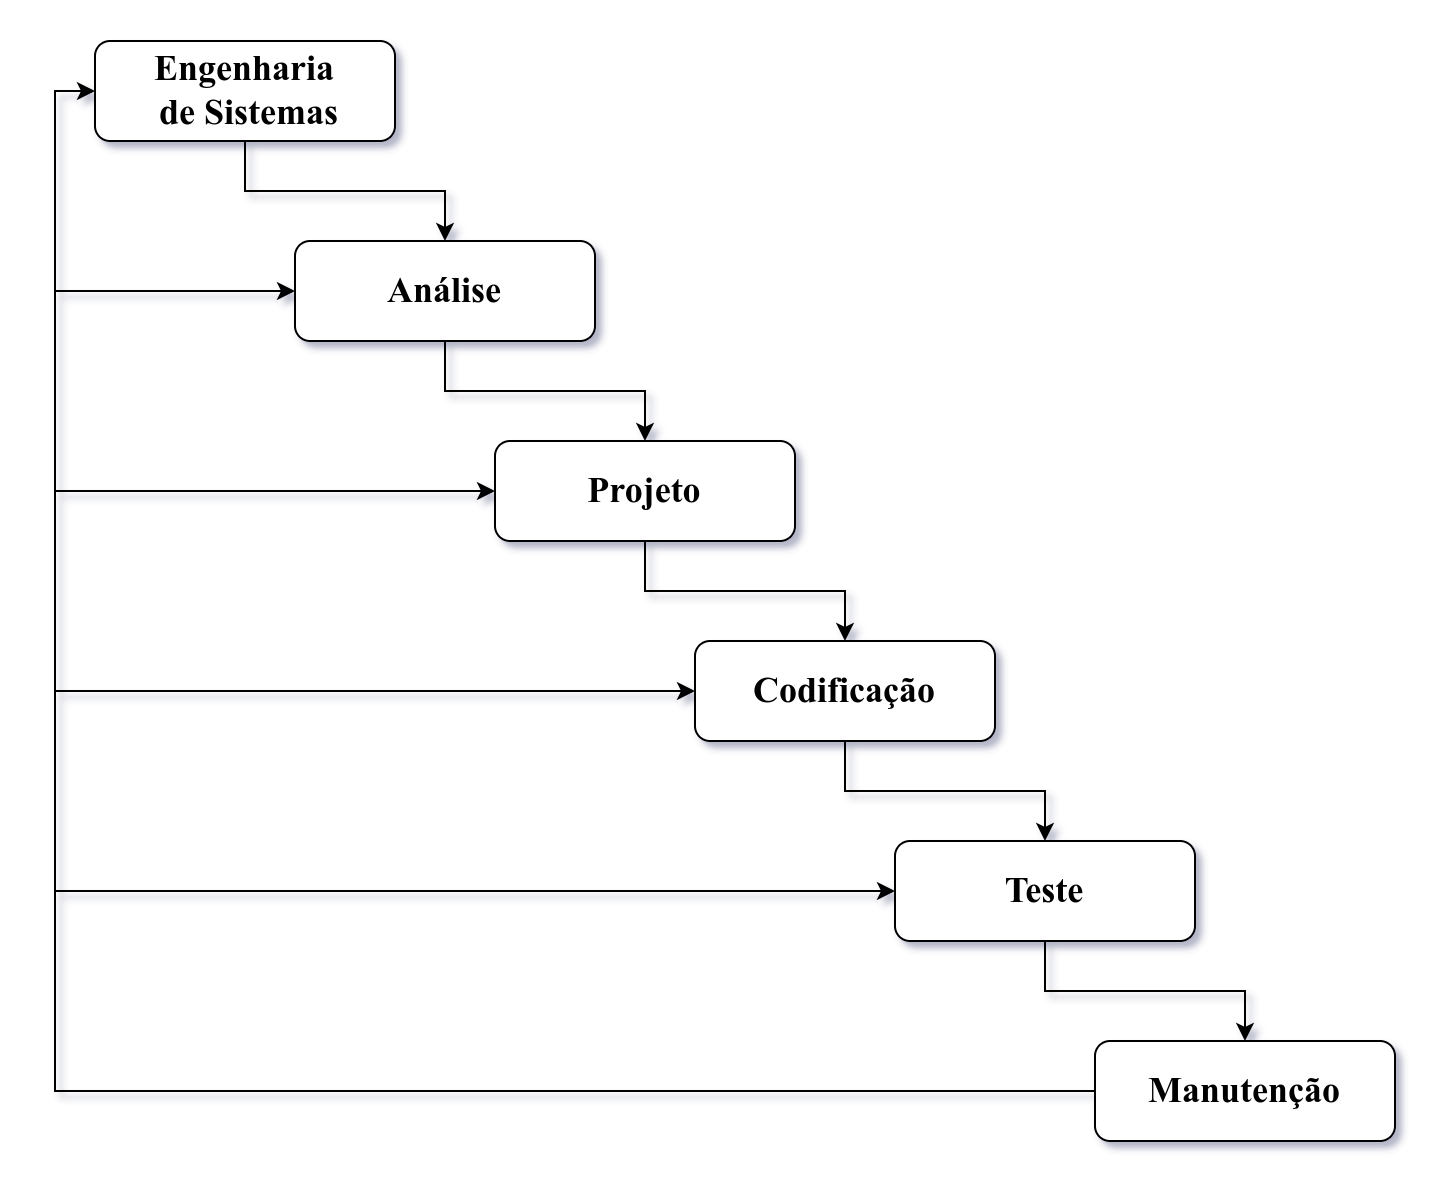
\includegraphics[scale=0.25]{waterfall.drawio.png}
    \caption{Desenvolvimento em Cascata}
\end{figure}

Esta estrutura é o que permite que o desenvolvimento ocorra de maneira crescente e parcial, onde cada adição, extensão,
 modificação ou remoção de componentes resulte na adaptação da documentação e código, voltando ao ponto de desenvolvimento 
 no qual a mudança ocorreu, garantindo assim uma maior estabilidade e qualidade de produto.

\subsubsection{Método de Trabalho}
O Método Ágil com SCRUM\footnote{
    Criado por \textbf{Jeff Sutherland} em 1990.
} foi empregado para orientar os desenvolvimentos dos diferentes processos presentes na estrutura do projeto. Utilizado também no mercado 
de trabalho, o método incorpora as atividades de levantamento de requisitos, análise, projetos \textit{(prototipação)}, 
implementação/evolução, e entrega.

As atividades individuais são organizadas em \textbf{Sprints}, que delimitam um certo período de 
tempo -- \textit{geralmente de uma a duas semanas} -- desde o início até o fim do processo.

\subsubsection{Divisão de Responsabilidades}
O projeto consta com dois membros, portanto, as atividades estão substituídas da seguinte maneira:

\paragraph{Chrystian M. Franklin}
\begin{itemize}
    	\item Planejamento e Estruturação do Projeto;
    	\item Controle do Versionamento;
    	\item Correção de Bugs e Otimizações;
    	\item Implementação de Casos de Testes Automatizados;
    	\item Desenvolvimento dos Aspectos Back-End; e
    	\item Desenvolvimento dos Aspectos Front-End.
\end{itemize}

\paragraph{Wellington E. Rodrigues}
\begin{itemize}
		\item Planejamento e Estrturação do Projeto;
    	\item Design e Padrões de Cores;
    	\item Organização e Distribuição de Atividades e Responsabilidades;
    	\item Construção de Documentação e Manuais;
   		\item Levantamento de Requisitos e Features Adicionais;
    	\item Controle do Versionamento; e
    	\item Construção de Diagramas e Protótipos Gráficos.

\end{itemize}

% --- Segment: Requirements ---
\section{Levantamento de Requisitos}
\textbf{Levantamente de Requisitos} é a prática onde se estuda e debate as funcionalidades que deverão ser contempladas no sistema, 
além das regras para tais funcionalidades e os cenários de implantação. Todo esse estudo, compreende na \textbf{Engenharia de Sistemas} 
que oferece suporte e abrange todas as atividades relacionadas à investigação, definição e delimitação de novos sistemas ou modificações.

Essa etapa é crucial no processo de desenvolvimento de software, no qual o engenheiro de requisitos, o analista de negócios, e 
o engenheiro de sistemas ou desenvolvedor de software trabalham juntos para identificar as necessidades e requisitos do cliente. Uma 
vez que os requisitos do sistema são identificados, os projetistas de sistemas estão prontos para criar a solução.

Na etapa de \textbf{Levantamento de Requisitos} temos a deinfição de três tipos de requisitos, onde cada um deles possuem suas 
características próprias. Os requisitos são:
\begin{itemize}
	\item Requisitos Funcionais;
	\item Requisitos Não-Funcionais; e
	\item Requisitos de Domínio.
\end{itemize}


\subsection{Requisitos Funcionais}
Os \textbf{Requisitos Funcionais} são aqueles que indicam quais as funcionalidades o sistema possuirá, ou seja, o que o sistema 
é capaz de executar e processar com as informações. Exemplos são:
\begin{itemize}
	\item Capacidade de cadastramento de usuários;
	\item Capacidade de geração de relatório mensal de vendas; e
	\item Capacidade de exportar os dados em arquivos.
\end{itemize}
Outros aspecto importante sobre os requisitos de domínio são: 
\begin{itemize}
	\item\textbf{Rastreabilidade:} entre os requisitos, ou seja, a capacidade de identificar quais requisitos estão 
	relacionados entre si, e quais requisitos são dependentes de outros requisitos;
	\item\textbf{Stakeholders:} aquele quem está diretamente ligado pu relacionado a funcionalidade em questão.
\end{itemize}


\subsection{Requisitos Não-Funcionais}
Os \textbf{Requisitos Não-Funcionais} são aqueles que quais as obrigações ou regras que devem ser aplicadas para que as 
funcionalidades descritas nos Requisitos Funcionais estejam em conformidade com a necessidade do cliente.
Outra aplicação dos \textbf{Requisitos Não-Funcionais} é quanto a limitação do sistema, ou seja, o que ele não deve fazer 
em hipótese alguma. Exemplos são:
\begin{itemize}
	\item Tempo execução de ações do sistema menor do que 2 segundos; e
	\item Compatibilidade do sistema com sistemas operacionais (caso uma aplicação desktop) ou com versões de 
	navegadores (caso uma aplicação web).
\end{itemize}


\subsection{Requisitos de Domínio}
Os \textbf{Requisitos de Domínio} são aqueles que buscam alinhar o domínio do cliente, ou seja, o ambiente/segmeto de 
mercado que está inserido e ao qual o \textit{software} desenvolvido será inserido. Exemplos são:
\begin{itemize}
	\item A geração de relatórios deve ser feita sempre filtrando pelo dados mais recentes e com maiores índices; e
	\item O sistema somente ficará disponível para emissões de notas em horário comercial.
\end{itemize}

% --- Segment: Data Flow Diagrams ---
\section{Diagrama de Fluxo de Dados}
Os \textbf{Diagramas de Fluxo de Dados} são os diagramas que representam como os dados percorrem por entre os processos e por quais processos. 
Cada Requisito Funcional deve apresentar um DFD (Diagrama de Fluxo de Dados) correspondente ao processo.

\section{Requisitos e DFDs}
\subsection{Requisitos Funcionais do Sistema}
\begin{figure}[H]
	\centering
	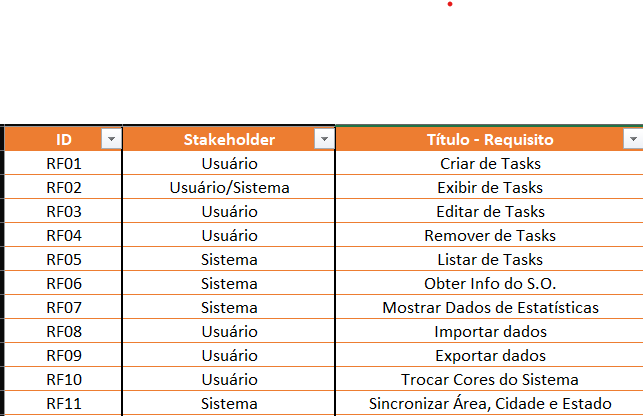
\includegraphics[scale=0.80]{requirements/functionals/requirements.png}
	\caption{Requisitos Funcionais do Sistema}
\end{figure}
\noindent Fonte: Os Autores.


Descrição de cada Requisito Funcional:
\begin{figure}[H]
	\centering
	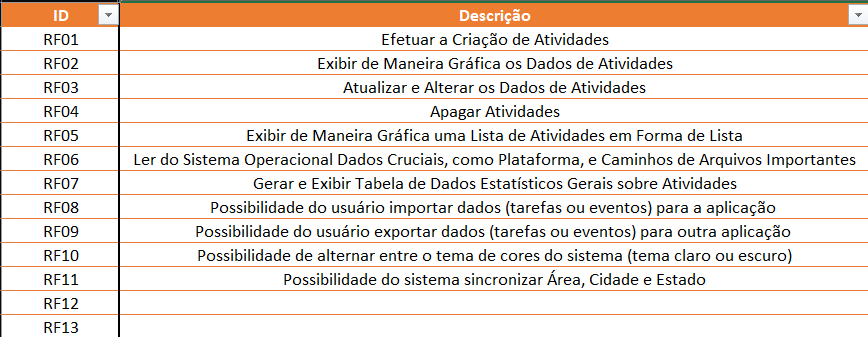
\includegraphics[scale=0.80]{requirements/functionals/description.png}
	\caption{Descrição dos Requisitos Funcionais do Sistema}
\end{figure}
\noindent Fonte: Os Autores.


\subsection{Requisitos Não-Funcionais do Sistema}
\begin{figure}[H]
	\centering
	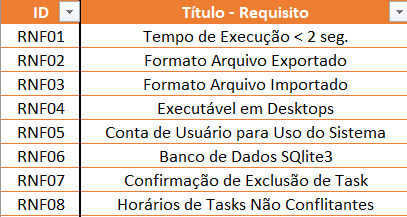
\includegraphics[scale=0.80]{requirements/not-functionals/not-functionals.png}
	\caption{Requisitos Não-Funcionais do Sistema}
\end{figure}
\noindent Fonte: Os Autores.


Descrição de cada Requisito Não-Funcional:
\begin{figure}[H]
	\centering
	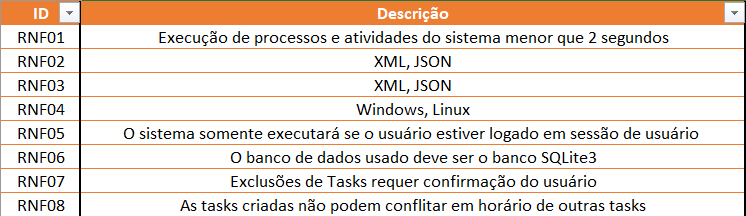
\includegraphics[scale=0.80]{requirements/not-functionals/description.png}
	\caption{Descrição dos Requisitos Não-Funcionais do Sistema}
\end{figure}
\noindent Fonte: Os Autores.


\subsection{Requisitos de Domínio do Sistema}
\begin{figure}[H]
	\centering
	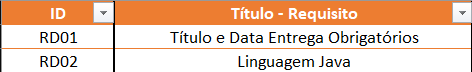
\includegraphics[scale=0.80]{requirements/domain/domain.png}
	\caption{Requisitos de Domínio do Sistema}
\end{figure}
\noindent Fonte: Os Autores.


Descrição de cada Requisito de Domínio:
\begin{figure}[H]
	\centering
	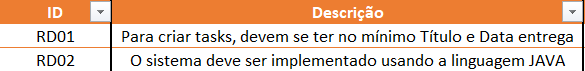
\includegraphics[scale=0.80]{requirements/domain/description.png}
	\caption{Descrição dos Requisitos de Domínio do Sistema}
\end{figure}
\noindent Fonte: Os Autores.

\pagebreak
\subsection{RF01 - Criar Tasks}
O sistema deve permitir que o usuário crie uma nova {Task}, onde o usuário deve informar o título da {Task}, a data 
de término da {Task}, sendo estes dois primeiros os dados obrigatórios para sua criação. Como dados opcionais, temos a 
data de início da {Task}, descrição da {Task}, repetição entre períodos e as tags da {Task}.
\begin{figure}[H]
	\centering
	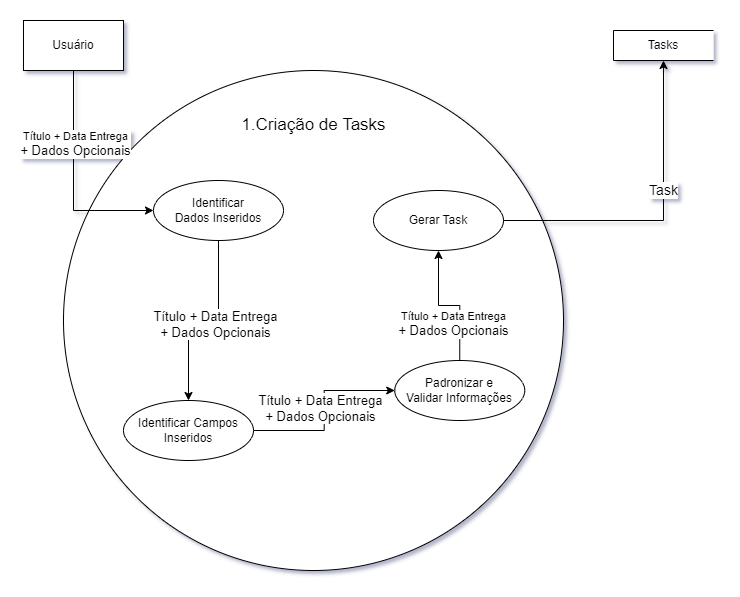
\includegraphics[scale=0.45]{DFDs/RF01.drawio.png}
	\caption{Diagrama de Fluxo de Dados do Requisito Funcional 01}
\end{figure}
\noindent Fonte: Os Autores.

\pagebreak
\subsection{RF02 - Exibir Tasks}
O sistema deve permitir que o usuário visualize todas as {Tasks} já existentes, onde o usuário pode vizualizar 
título, data de início, data de término, descrição, repetição entre períodos e as tags da {Task}. Além disso, o 
sistema deve fornecer essa exibição assim que o usuário abrir o sistema. Ou seja, dois \textit{stakesholders} 
podem ser identificados: usuário e o sistema.
\begin{figure}[H]
	\centering
	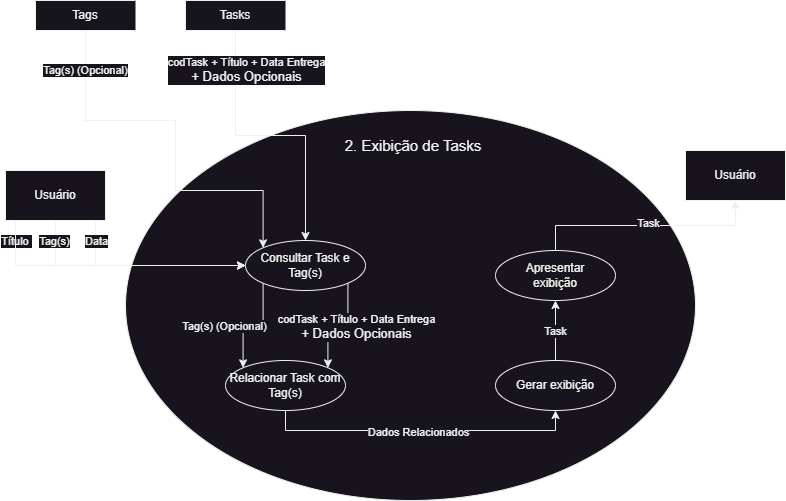
\includegraphics[scale=0.45]{DFDs/RF02.drawio.png}
	\caption{Diagrama de Fluxo de Dados do Requisito Funcional 02}
\end{figure}
\noindent Fonte: Os Autores.

\pagebreak
\subsection{RF03 - Editar Tasks}
O sistema deve permitir que o usuário edite uma {Task} já existente, onde o usuário deve informar o 
título da {Task}, a data de término da {Task}, sendo estes dois primeiros os dados obrigatórios 
para sua criação. Como dados opcionais, temos a data de início da {Task}, descrição da {Task}, 
repetição entre períodos e as tags da {Task}.
\begin{figure}[H]
	\centering
	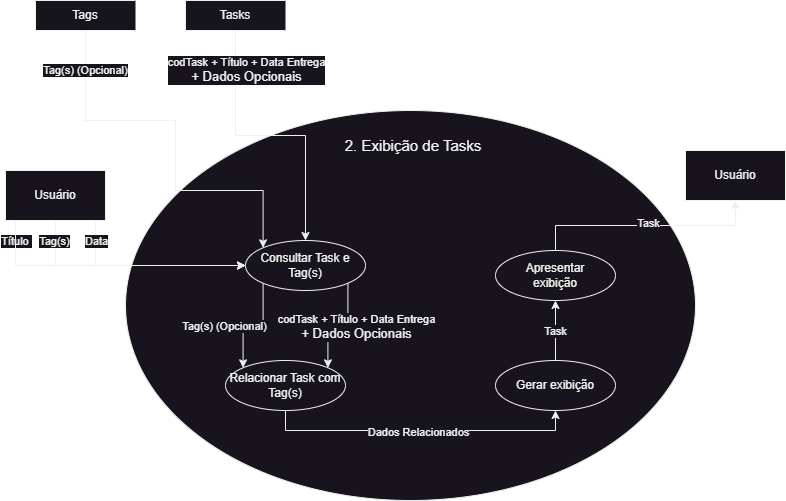
\includegraphics[scale=0.45]{DFDs/RF02.drawio.png}
	\caption{Diagrama de Fluxo de Dados do Requisito Funcional 03}
\end{figure}
\noindent Fonte: Os Autores.

\pagebreak
\subsection{RF04 - Excluir Tasks}
O sistema deve permitir que o usuário exclua uma {Task} já existente, onde o usuário deve informar o título 
da {Task} a ser excluída.
\begin{figure}[H]
	\centering
	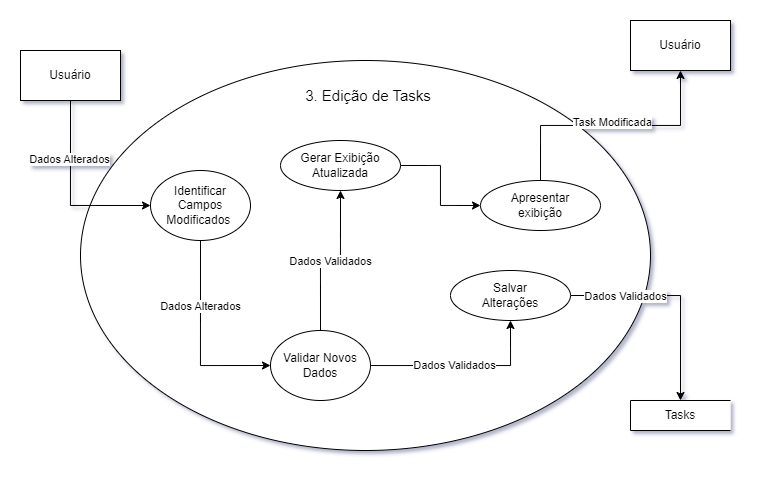
\includegraphics[scale=0.45]{DFDs/RF03.drawio.png}
	\caption{Diagrama de Fluxo de Dados do Requisito Funcional 04}
\end{figure}
\noindent Fonte: Os Autores.

\pagebreak
\subsection{RF05 - Listar Tags}
O sistema deve listar todas as {Tags} já existentes, em ordem de mais recentes para mais antigas.
\begin{figure}[H]
	\centering
	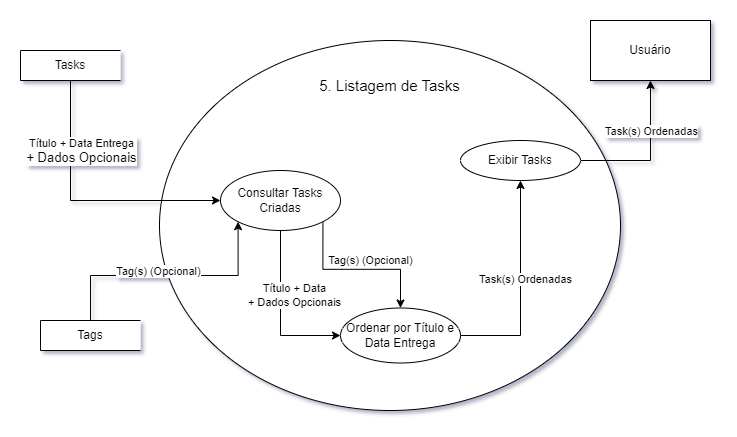
\includegraphics[scale=0.45]{DFDs/RF05.drawio.png}
	\caption{Diagrama de Fluxo de Dados do Requisito Funcional 05}
\end{figure}
\noindent Fonte: Os Autores.

\pagebreak
\subsection{RF06 - Obter Infor do Sistema Operacional}
O sistema deve obter informações do sistema operacional, com qual é por exemplo.
\begin{figure}[H]
	\centering
	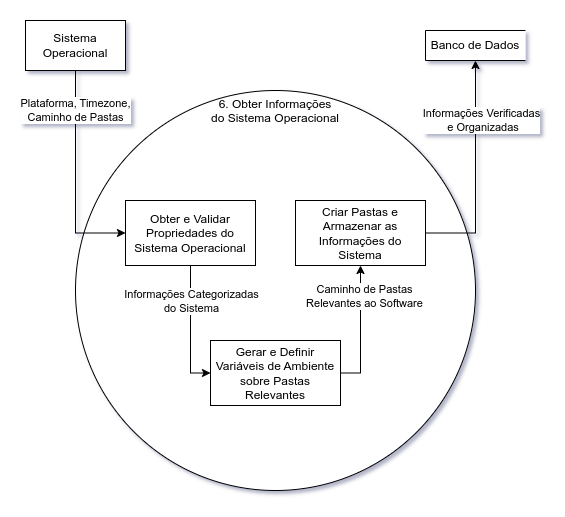
\includegraphics[scale=0.45]{DFDs/RF06.drawio.png}
	\caption{Diagrama de Fluxo de Dados do Requisito Funcional 06}
\end{figure}
\noindent Fonte: Os Autores.

\pagebreak
\subsection{RF07 - Mostra Dados de Estatísticas}
O sistema deve mostrar dados de estatísticas, sendo o número de task criadas, concluídas, programadas e atrasadas.
\begin{figure}[H]
	\centering
	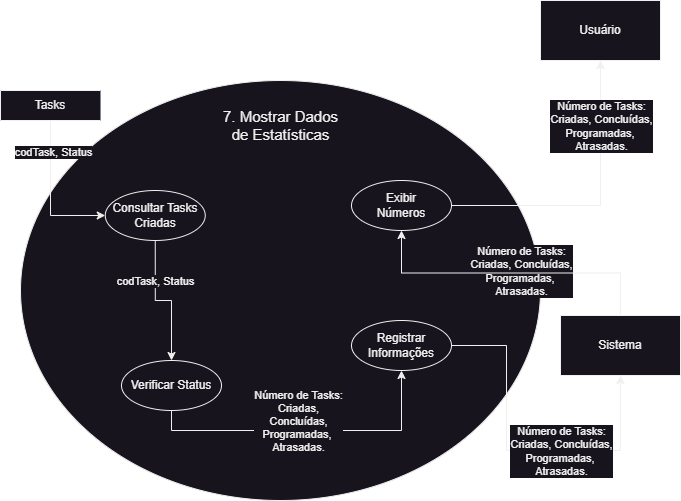
\includegraphics[scale=0.45]{DFDs/RF07.drawio.png}
	\caption{Diagrama de Fluxo de Dados do Requisito Funcional 07}
\end{figure}
\noindent Fonte: Os Autores.

\pagebreak
\subsection{RF08 - Importar Dados}
O sistema deve ser capaz de importar dados externos, sendo eles por arquivos nos formatos \textbf{.xml} e \textbf{.json}.
\begin{figure}[H]
	\centering
	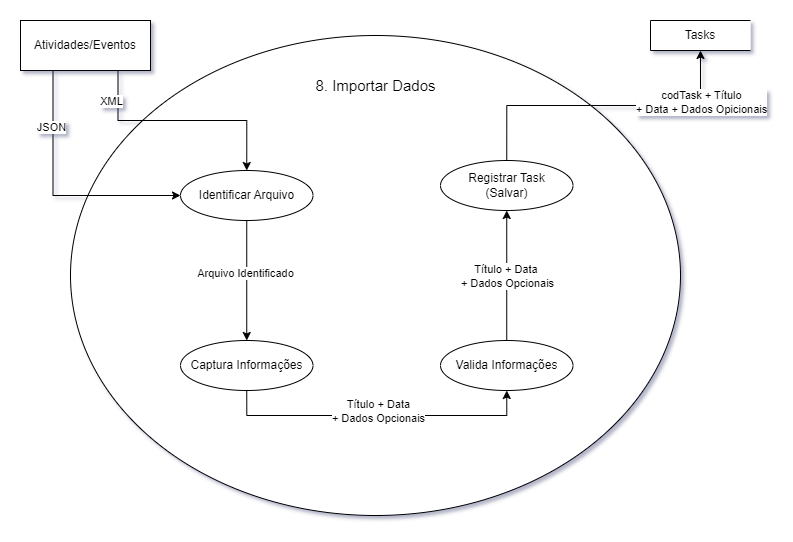
\includegraphics[scale=0.45]{DFDs/RF08.drawio.png}
	\caption{Diagrama de Fluxo de Dados do Requisito Funcional 08}
\end{figure}
\noindent Fonte: Os Autores.

\pagebreak
\subsection{RF09 - Exportar Dados}
O sistema decve ser capaz de exportar os dados internos, ou seja, as Tasks cadastradas no banco. A exportação deve possibilitar 
em arquivo de formato \textbf{.json} e \textbf{.xml}.
\begin{figure}[H]
	\centering
	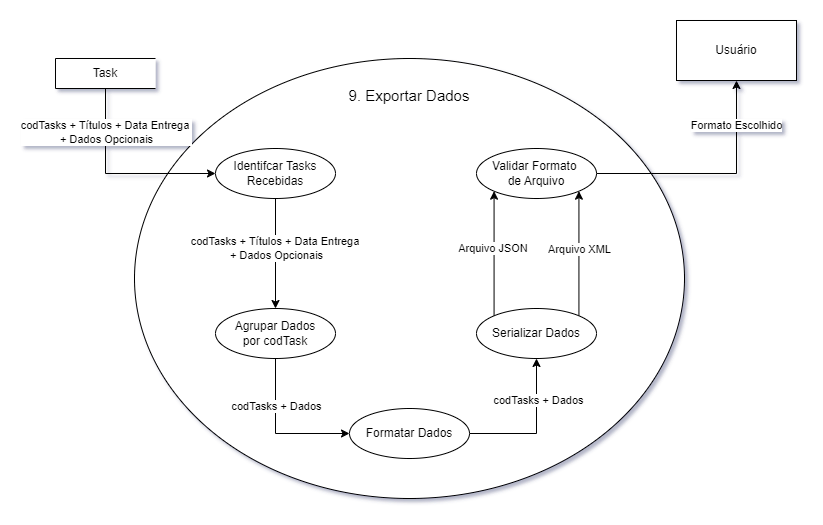
\includegraphics[scale=0.45]{DFDs/RF09.drawio.png}
	\caption{Diagrama de Fluxo de Dados do Requisito Funcional 09}
\end{figure}
\noindent Fonte: Os Autores.

\pagebreak
\subsection{RF10 - Trocar Tema}
O sistema deve ser capaz de trocar o tema, sendo eles o tema claro e o tema escuro.
\begin{figure}[H]
	\centering
	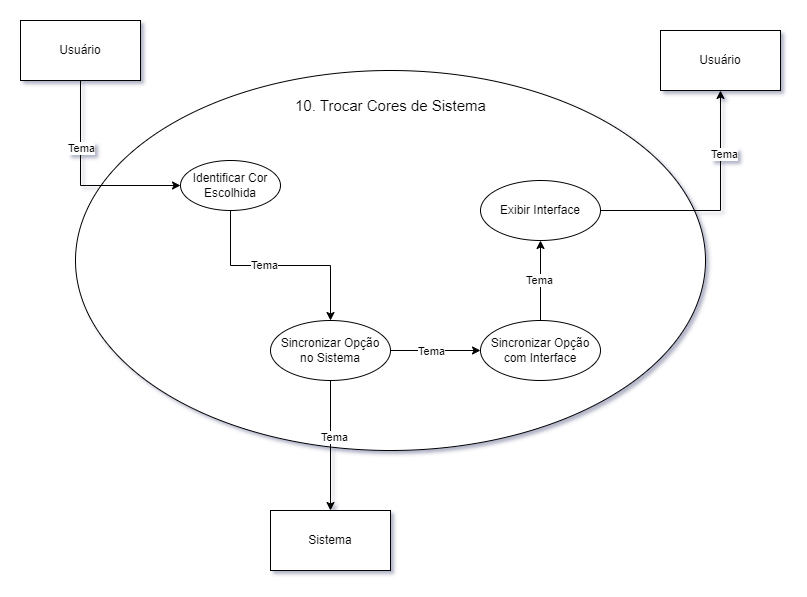
\includegraphics[scale=0.45]{DFDs/RF10.drawio.png}
	\caption{Diagrama de Fluxo de Dados do Requisito Funcional 10}
\end{figure}
\noindent Fonte: Os Autores.

\pagebreak
\subsection{RF11 - Sincronizar Localidade}
O sistema deve ser capaz de sincronizar a localidade física do usuário com o sistema, ou seja, sincronizar cidade e estado.
\begin{figure}[H]
	\centering
	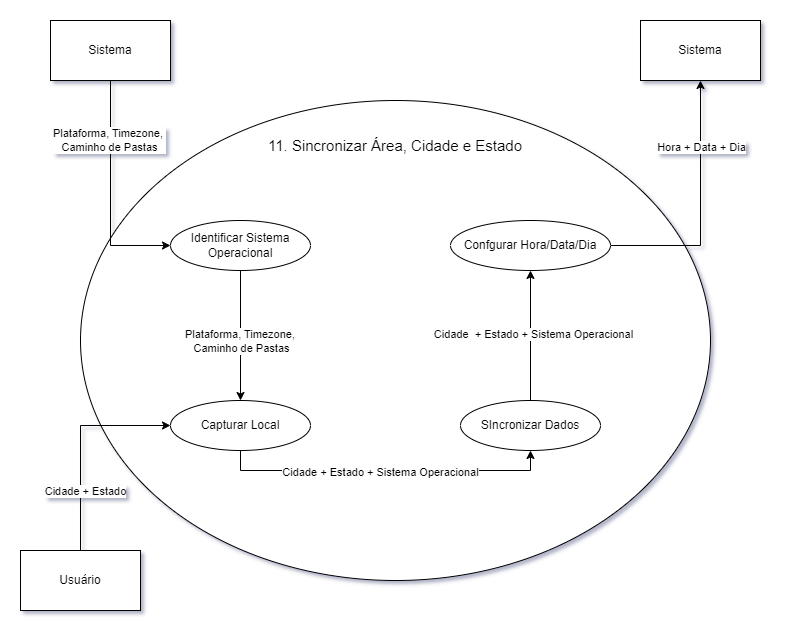
\includegraphics[scale=0.45]{DFDs/RF11.drawio.png}
	\caption{Diagrama de Fluxo de Dados do Requisito Funcional 11}
\end{figure}
\noindent Fonte: Os Autores.

\pagebreak
\section{Dicionário de Dados}
O \textbf{Dicionário de Dados} é o documento ao qual é representado os tipos de dados, quais são eles e como serão 
representados dentro do sistema. Abaixo, segue uma tabela que demonstra os tipos de dados e suas representações:

\begin{table}[H]
	\noindent
	\begin{tabular}{|l|}
		\hline
			\textbf{task =} @ID + Título + Data de Entrega + (Descrição) + (Data de início) + (\{Tag\})\\ \hline
			\textbf{título =} 40\{texto\} \\ \hline
			\textbf{descrição =} 400\{texto\} \\ \hline
			\textbf{data de Vencimento =} 10[0-9|/] \\ \hline
			\textbf{data de Inicio =} 10[0-9|/] \\ \hline
			\textbf{tag =} 12[A-Z|a-z|À-Ù|à-ù|Á-Ú|á-ú|0-9| ] \\ \hline
			\textbf{texto =} [A-Z|a-z|À-Ù|à-ù|Á-Ú|á-ú|0-9|'|,|-|.|/| ] \\ \hline
	\end{tabular}
	\caption{Tipos de Dados e suas Representações}
\end{table}

% --- Segment: Design & Colors---
% --- Segment: Color Palette ---
\pagebreak
\section{Paleta de Cores do Sistema}
A paleta de cores do sistema é o conjunto de cores que serão utilizadas no sistema, tanto para o tema claro quanto 
para o tema escuro. É importante destacar que as cores do sistema foram escolhidas usando como base seu possíveis 
significados e o que elas poderiam significar para o usuário final, em diferentes situações e processos dentro do sistema. 

\subsection{Sistema de Cores}
Cada cor pode representar um emoção e expressar um significado quando se diz respeito a experiência do usuário. Expressar uma 
mensagem de forma adequada através das cores pode ser o elemento crucial que distingue o êxito do fracasso em um projeto. (“Medium”, [s.d.])

Logo, com objetivo de aplicar nossa identidade, além de passar uma boa experiência ao usuário, foram escolhidas as seguintes cores:

\subsection{Cores do Tema Claro}
\begin{itemize}
	\item \textbf{Branco} \#FFFFFF. Aplicação: \textit{Background} do JFrame principal. Além de fundo para os campos de \textit{input} e \textit{textarea} 
	situados nos JPanels com fundo cinza;
	\item \textbf{Cinza:} \#E4DEDE. AplicaçãO: \textit{Background} dos campos de \textit{input} e \textit{textarea} situados na barra de navegação;
	\item \textbf{Preto:} \#000000. Aplicação: Cores para textos e ícones;
	\item \textbf{Laranja:} \#FF3D00; Aplicação: \textit{Background} dos botões de salvar e linhas para voltar e cancelar, borda de JPanels 
	para destaque e detalhes mínimos de números no calendário;
	\item \textbf{Azul:} \#4646B9; Aplicação: \textit{Background} das Tags;
	\item \textbf{Azul 2:} \#0500FF; Aplicação: Linhas de destaque para seções, além de bordas para JPanels e detalhes mínimos;
	\item \textbf{Vermelho:} \#FF0000; Aplicação: Linhas do ícone de lixeira para exclusão de Tasks; e
	\item \textbf{Verde:} \#00FF00; Aplicação: Linhas do ícone de conclusão de Tasks.
\end{itemize}

\subsection{Cores do Tema Escuro}
\begin{itemize}
	\item \textbf{Preto:} \#000000. Aplicação: \textit{Background} do JFrame principal e para textos e ícones;
	\item \textbf{Branco} \#FFFFFF. Aplicação: \textit{Background} dos JPanels, além de fundo para os campos de \textit{input} e \textit{textarea} 
	situados na barra de navegação;
	\item \textbf{Cinza:} \#E4DEDE. AplicaçãO: \textit{Background} dos campos de \textit{input} e \textit{textarea} situados nos JPanels com fundo branco;
	\item \textbf{Laranja:} \#FF3D00; Aplicação: \textit{Background} dos botões de salvar e linhas para voltar e cancelar, borda de JPanels para 
	destaque e detalhes mínimos de números no calendário;
	\item \textbf{Azul:} \#4646B9; Aplicação: \textit{Background} das Tags e cor de seleção para \textit{Radio Buttons};
	\item \textbf{Azul 2:} \#0500FF; Aplicação: Linhas de destaque para seções, além de bordas para JPanels e detalhes mínimos;
	\item \textbf{Vermelho:} \#FF0000; Aplicação: Linhas do ícone de lixeira para exclusão de Tasks; e
	\item \textbf{Verde:} \#00FF00; Aplicação: Linhas do ícone de conclusão de Tasks.
	
\end{itemize}

\pagebreak
\section{Design}
% --- Segment: Prototypes ---
\subsection{Protótipos}
Prototipar é o processo ao qual uma versão básica do sistema, a fim de vizualizar qual seria o funcionamento do sistema ou que 
ele de fato poderia oferecer ao usuário final quanto a sua usabilidade do sistema, quanto as ferramentas e funcionalidade alinhadas 
na etapa de \textbf{Engenharia de Sistemas}, além de apresentar, o mais fielmente possível, os aspectos do front-end do sistema 
ou \textit{desing} das telas e relacionados.

Quanto ao funcionamento pensado, nossos sistema apresentaria todas as telas por meio de JPanels\footnote{
	Ferramenta de Organização de Painéis disponível no uso do Java Swing
}, a não ser a tela principal, que seria aplicado o uso de JFrames\footnote{
	Ferramenta de Organização de Telas (Frames) disponível no uso do Java Swing
}. A troca entre telas seria aplicada dinamicamente, de modo que a cada ação do usuário - ao clicar em um botão por exemplo - a 
tela correspondente seria aplicada sobre a tela atual, substituindo. Tal uso forneceria uma melhor usabilidade para o usuário, 
sem precisar se preocupar com a organização das telas no momento de inicialzação a cada evento.

\subsection{Tela Principal}
A \textbf{Tela Principal} seria o JFrame ao qual sempre seria atualizado os JPanels para cada ação correspondente do usuário, logo, 
os únicos componentes ou o único grupo de elementos seria a barra superior de navegação e pesquisa, presente em todo momento e em 
qualquer ação do sistema.

\pagebreak
\subsubsection{Tema Claro}
Telas com tema claro são aquelas que apresentam cores mais claras, como o branco, o cinza claro, o azul claro, entre outros. 
A ideia de um tema claro é a de que o usuário possa utilizar o sistema em ambientes com iluminação mais forte, como em ambientes 
externos, por exemplo.

\begin{itemize}
	\item Tela Principal
	\begin{figure}[H]
		\centering
		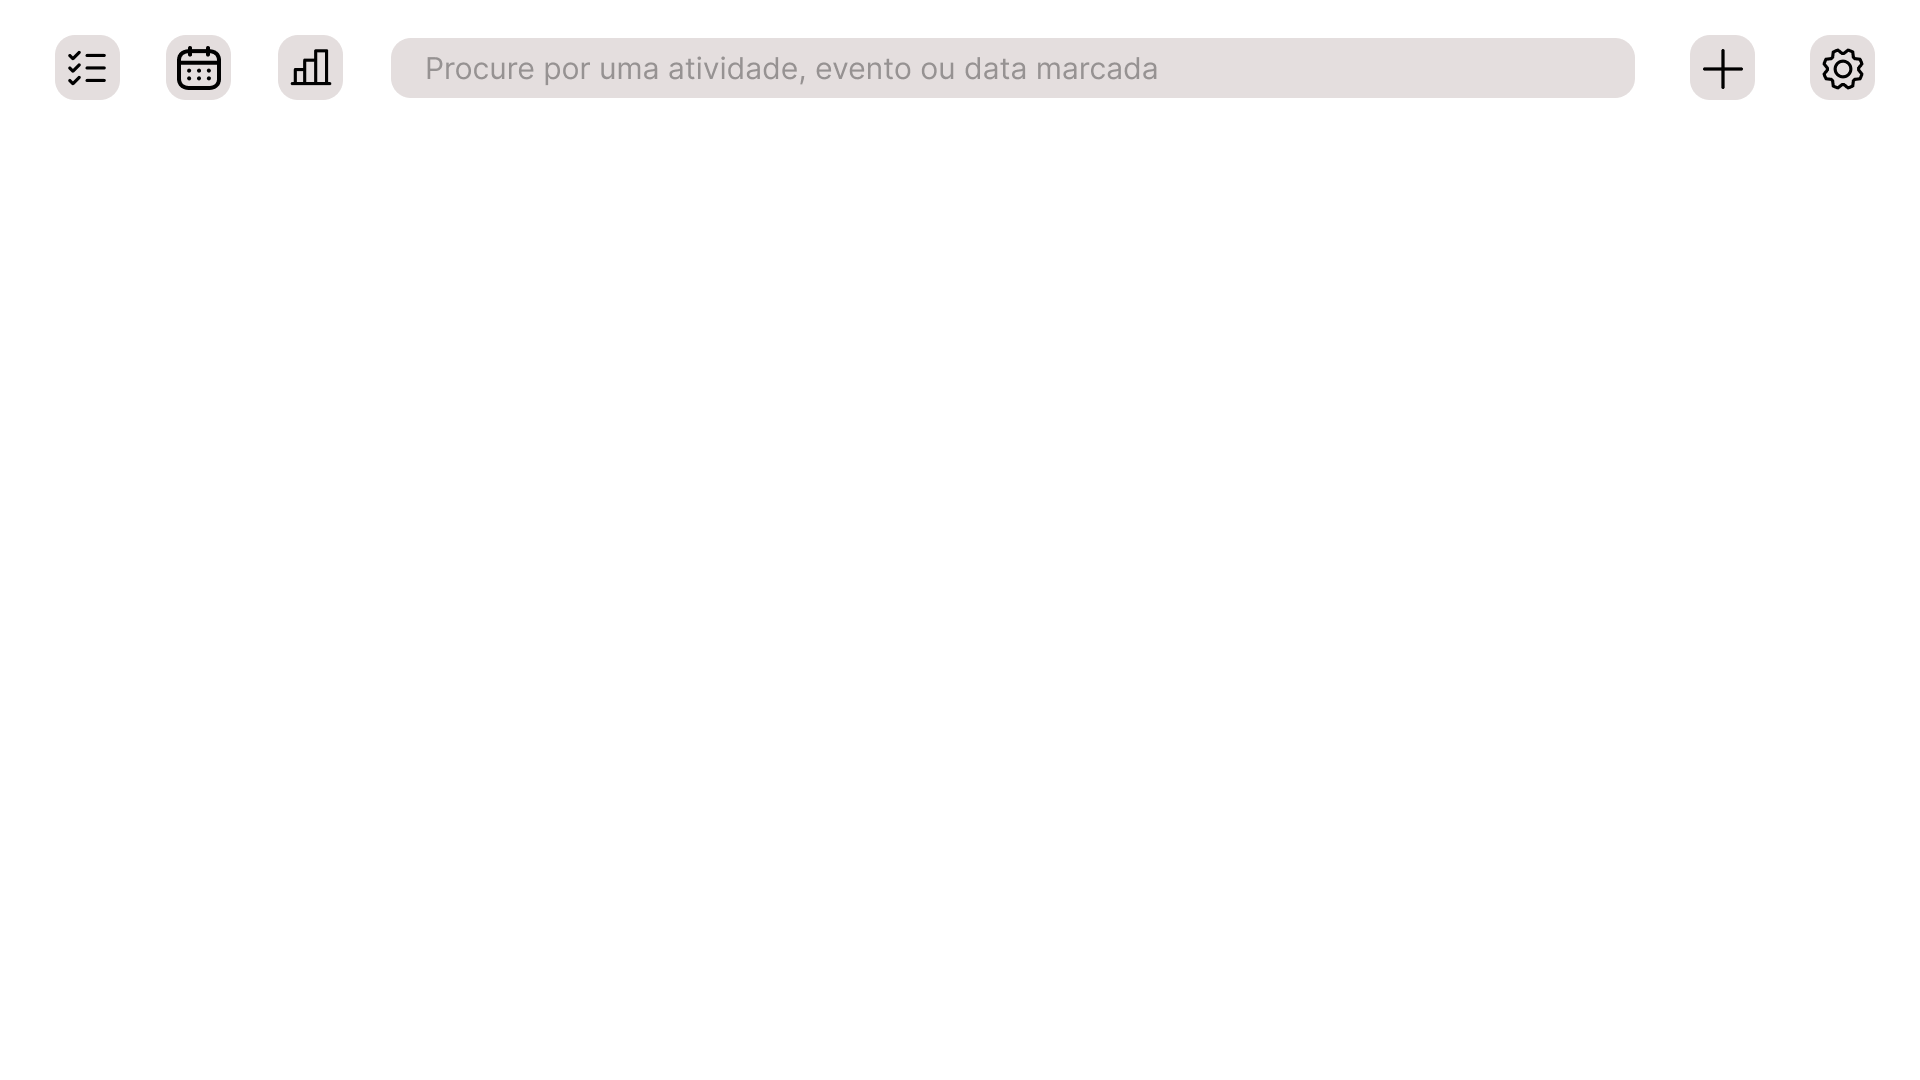
\includegraphics[scale=0.19]{prototypes/white/Main Window.png}
		\caption{JFrame principal - Modo Claro}
	\end{figure}
	\noindent Fonte: Os Autores.

	\item Calendário de Tasks
	\begin{figure}[H]
		\centering
		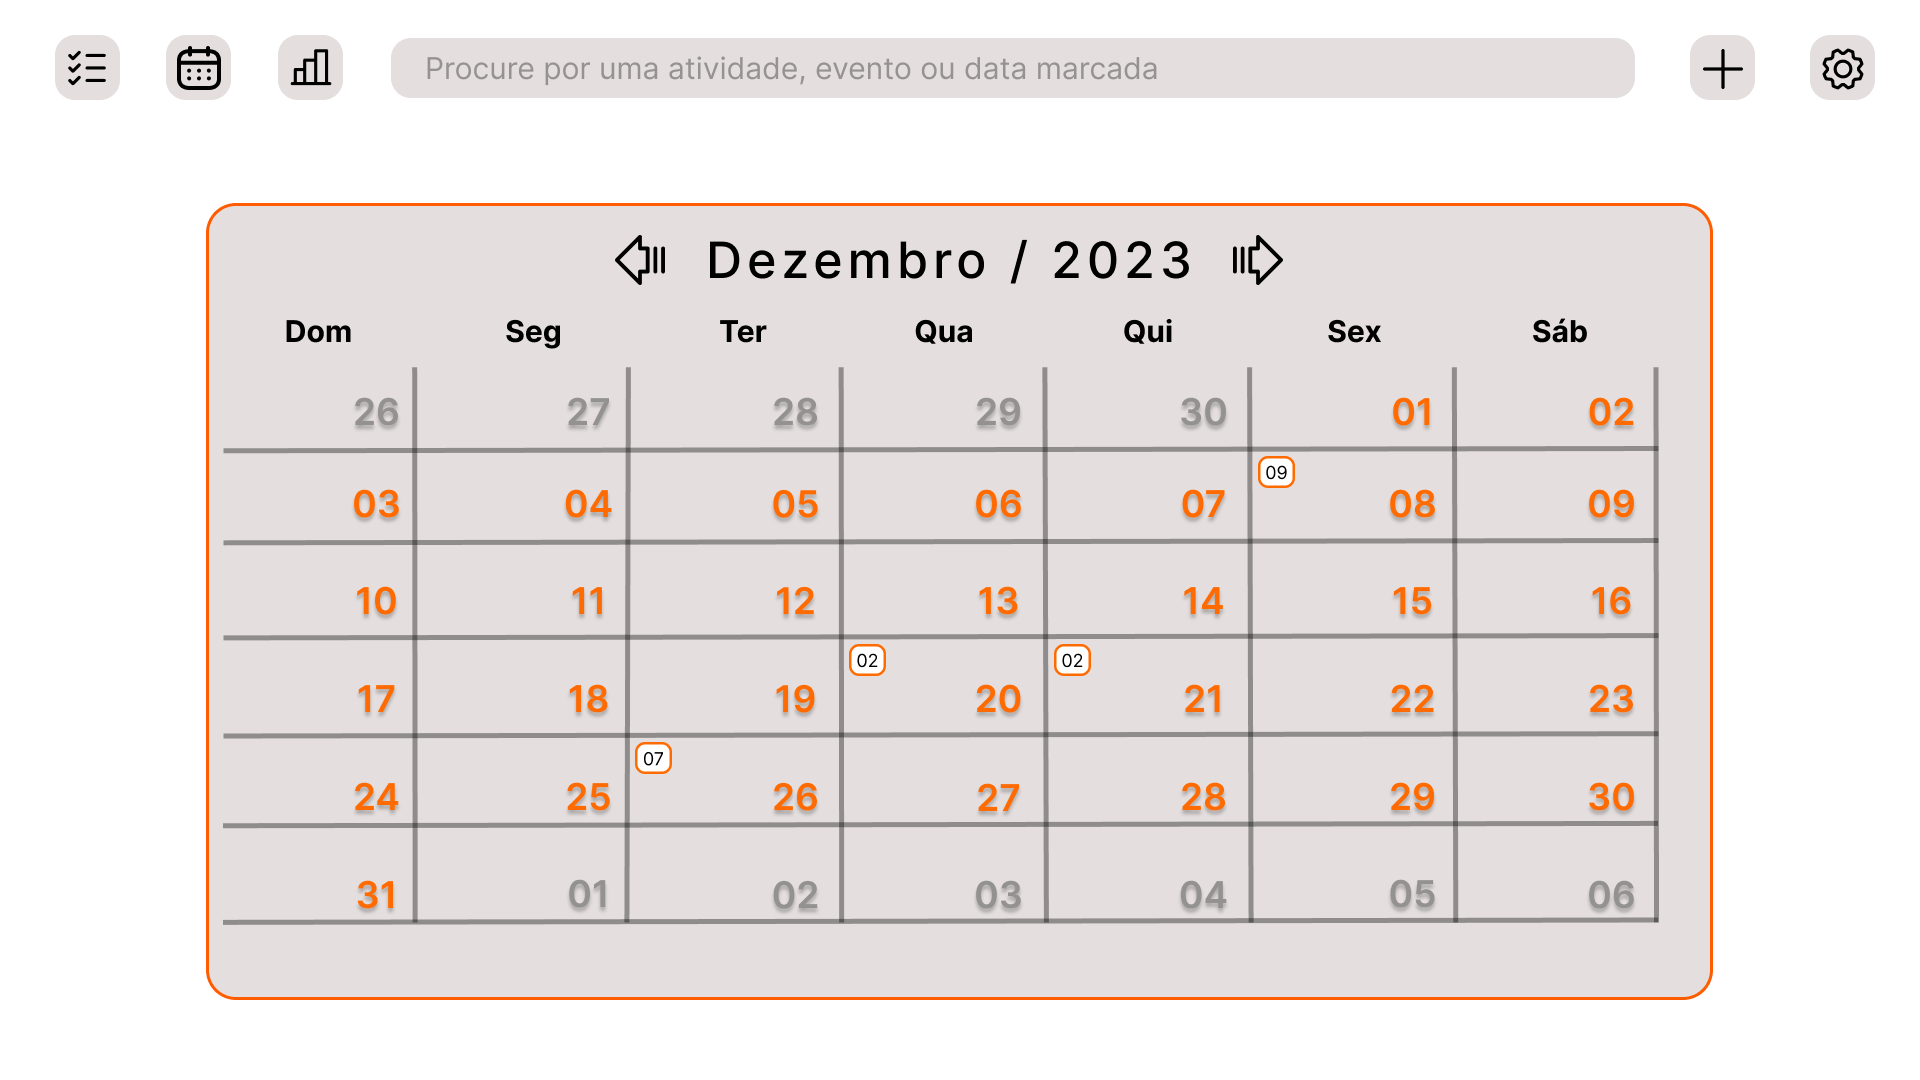
\includegraphics[scale=0.19]{prototypes/white/Calendar Panel Window.png}
		\caption{JPanel Calendário - Modo Claro}
	\end{figure}	
	\noindent Fonte: Os Autores.

	\pagebreak
	\item Estatísticas Gerais
	\begin{figure}[H]
		\centering
		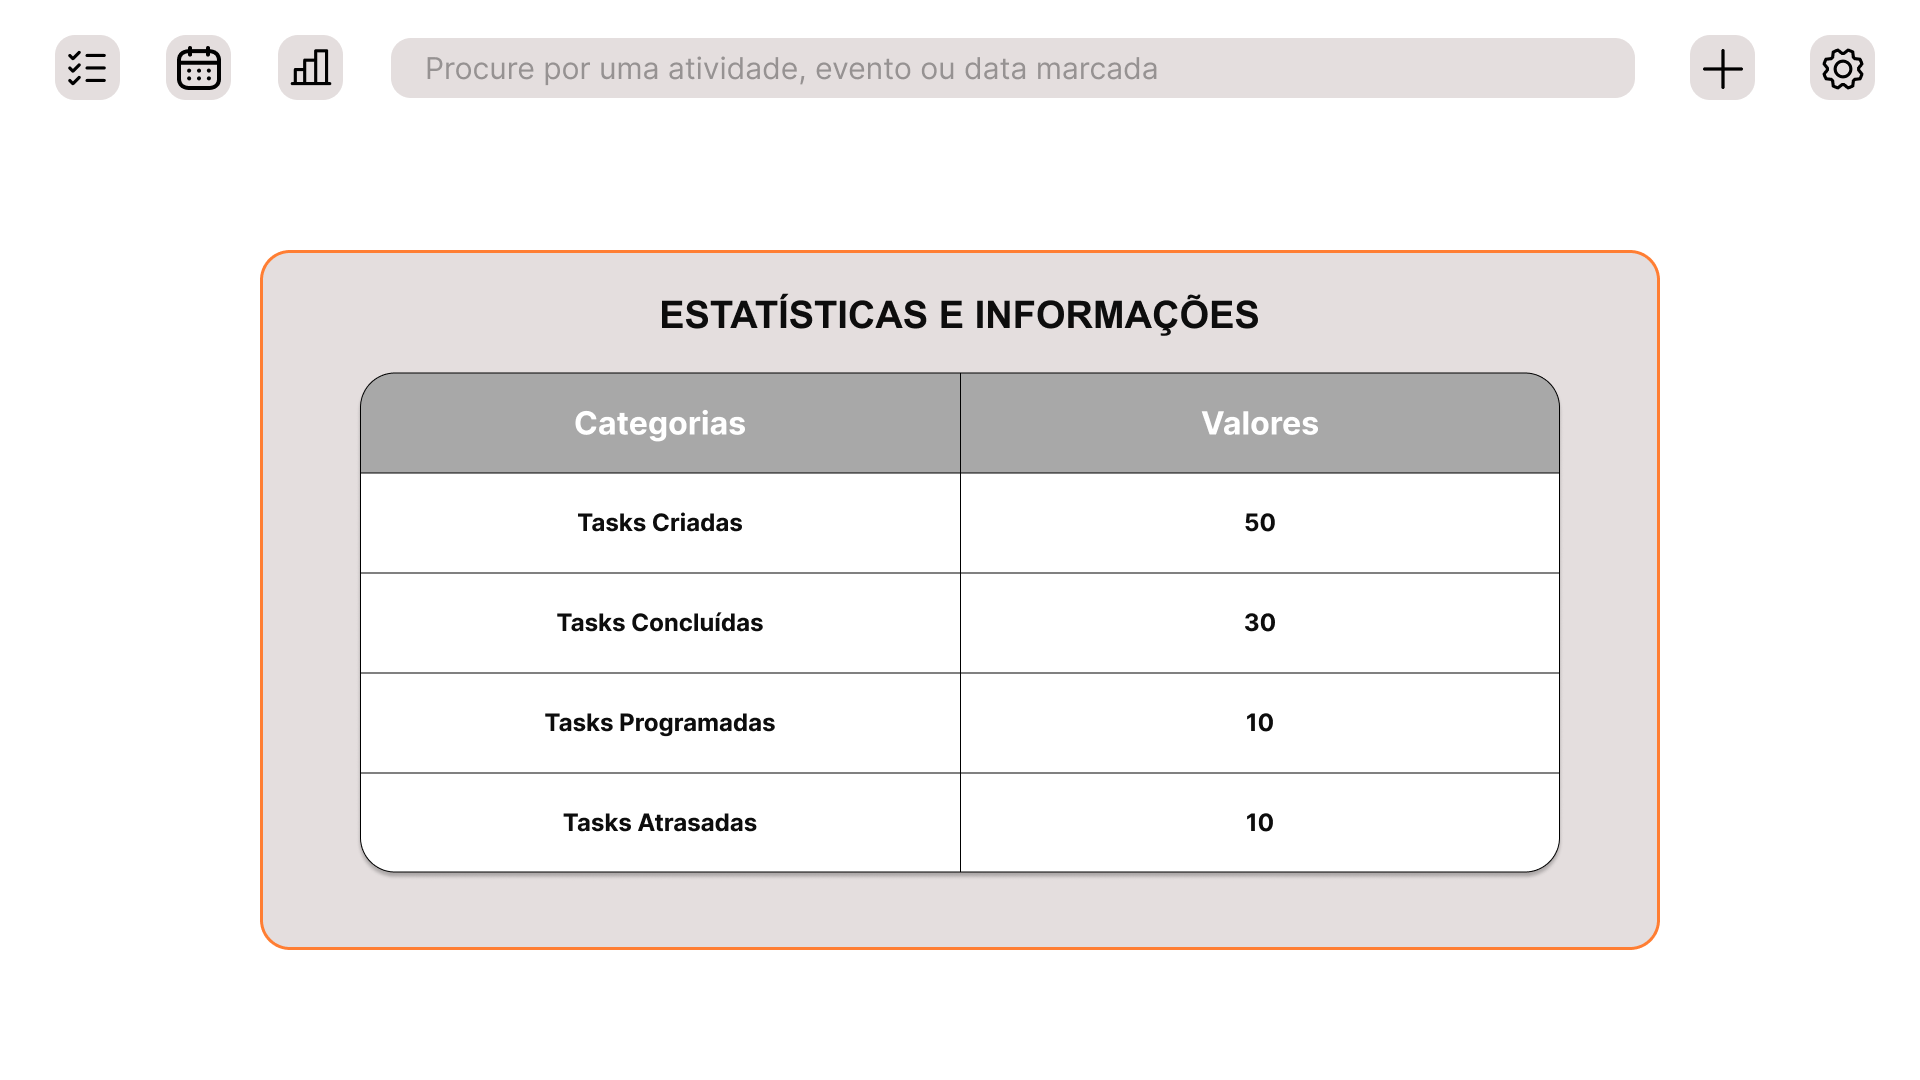
\includegraphics[scale=0.19]{prototypes/white/Stats Panel Window.png}
		\caption{JPanel de Informações e Estatísticas - Modo Claro}
	\end{figure}
	\noindent Fonte: Os Autores.

	\item Tela de Configuração
	\begin{figure}[H]
		\centering
		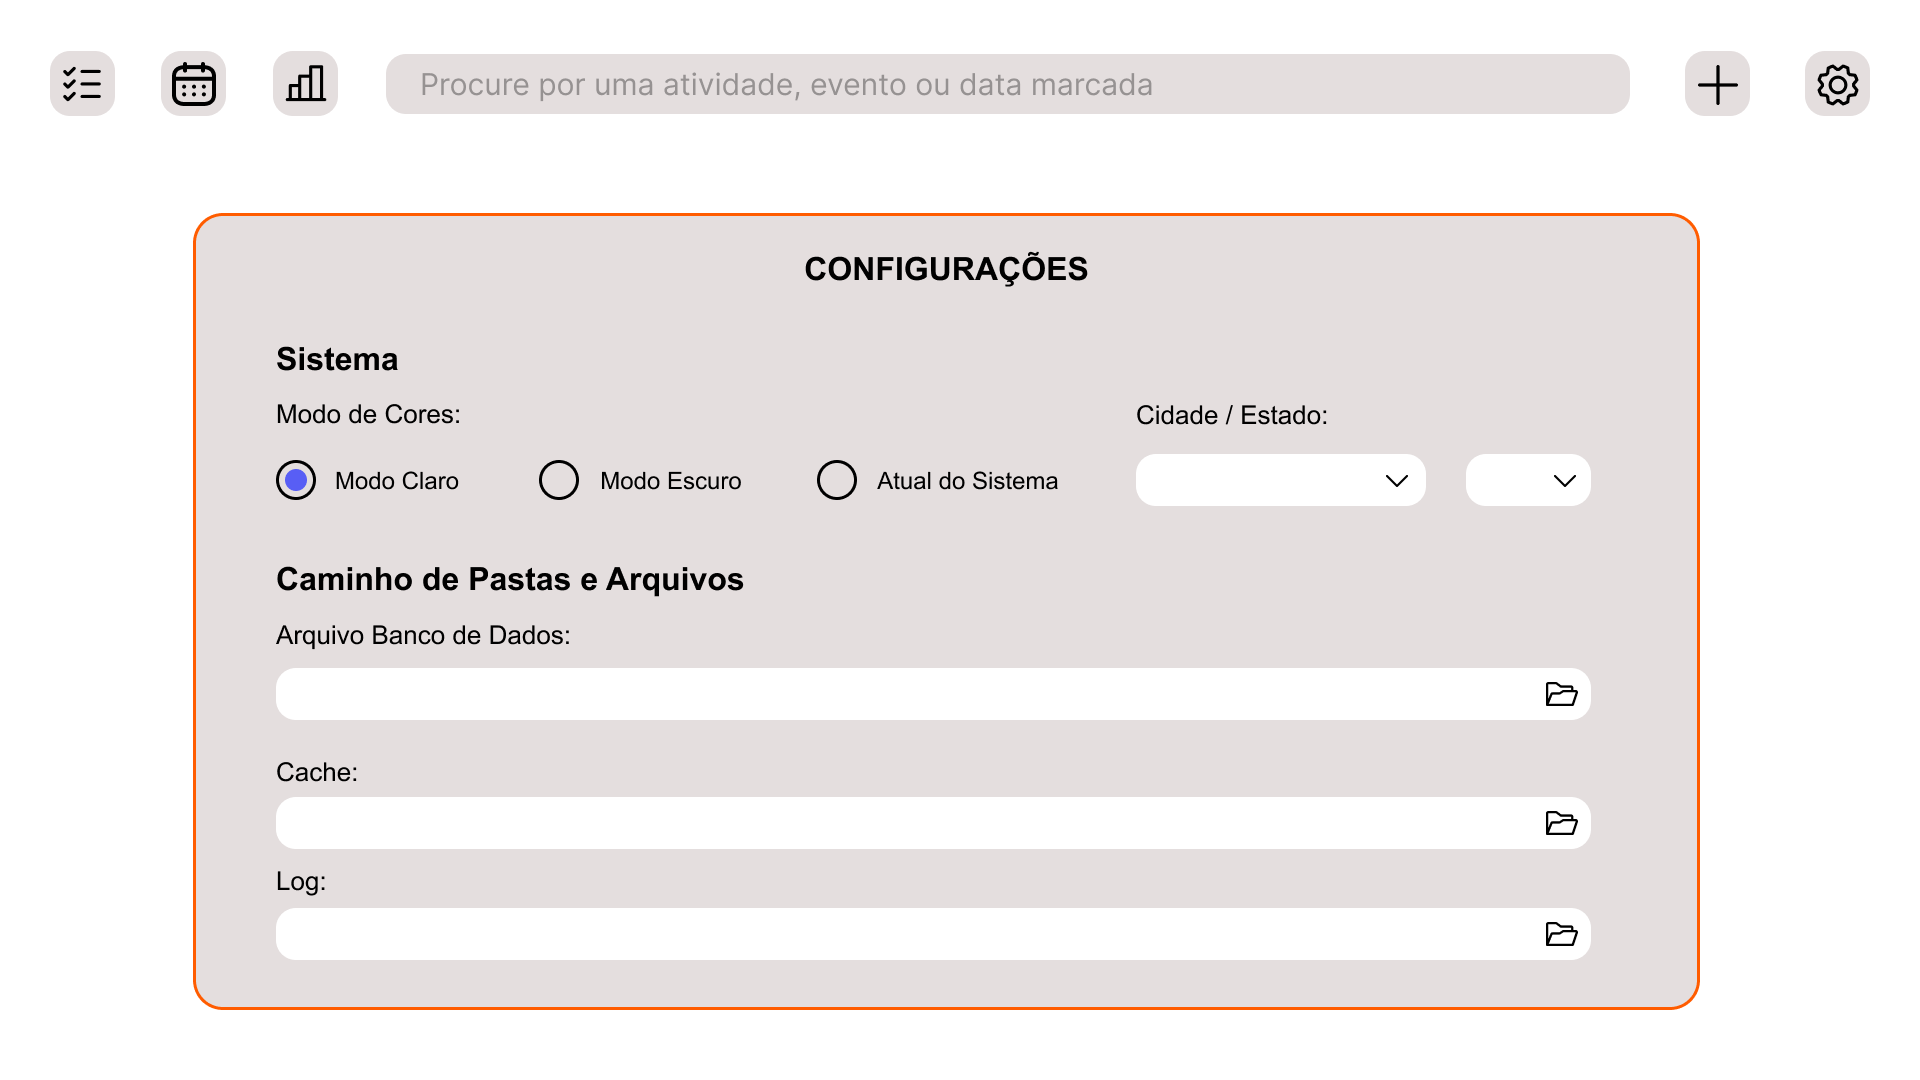
\includegraphics[scale=0.19]{prototypes/white/Config Panel Window.png}
		\caption{JPanel de Configurações - Modo Claro}
	\end{figure}
	\noindent Fonte: Os Autores.

	\pagebreak
	\item Tela de Adição de Tasks
	\begin{figure}[H]
		\centering
		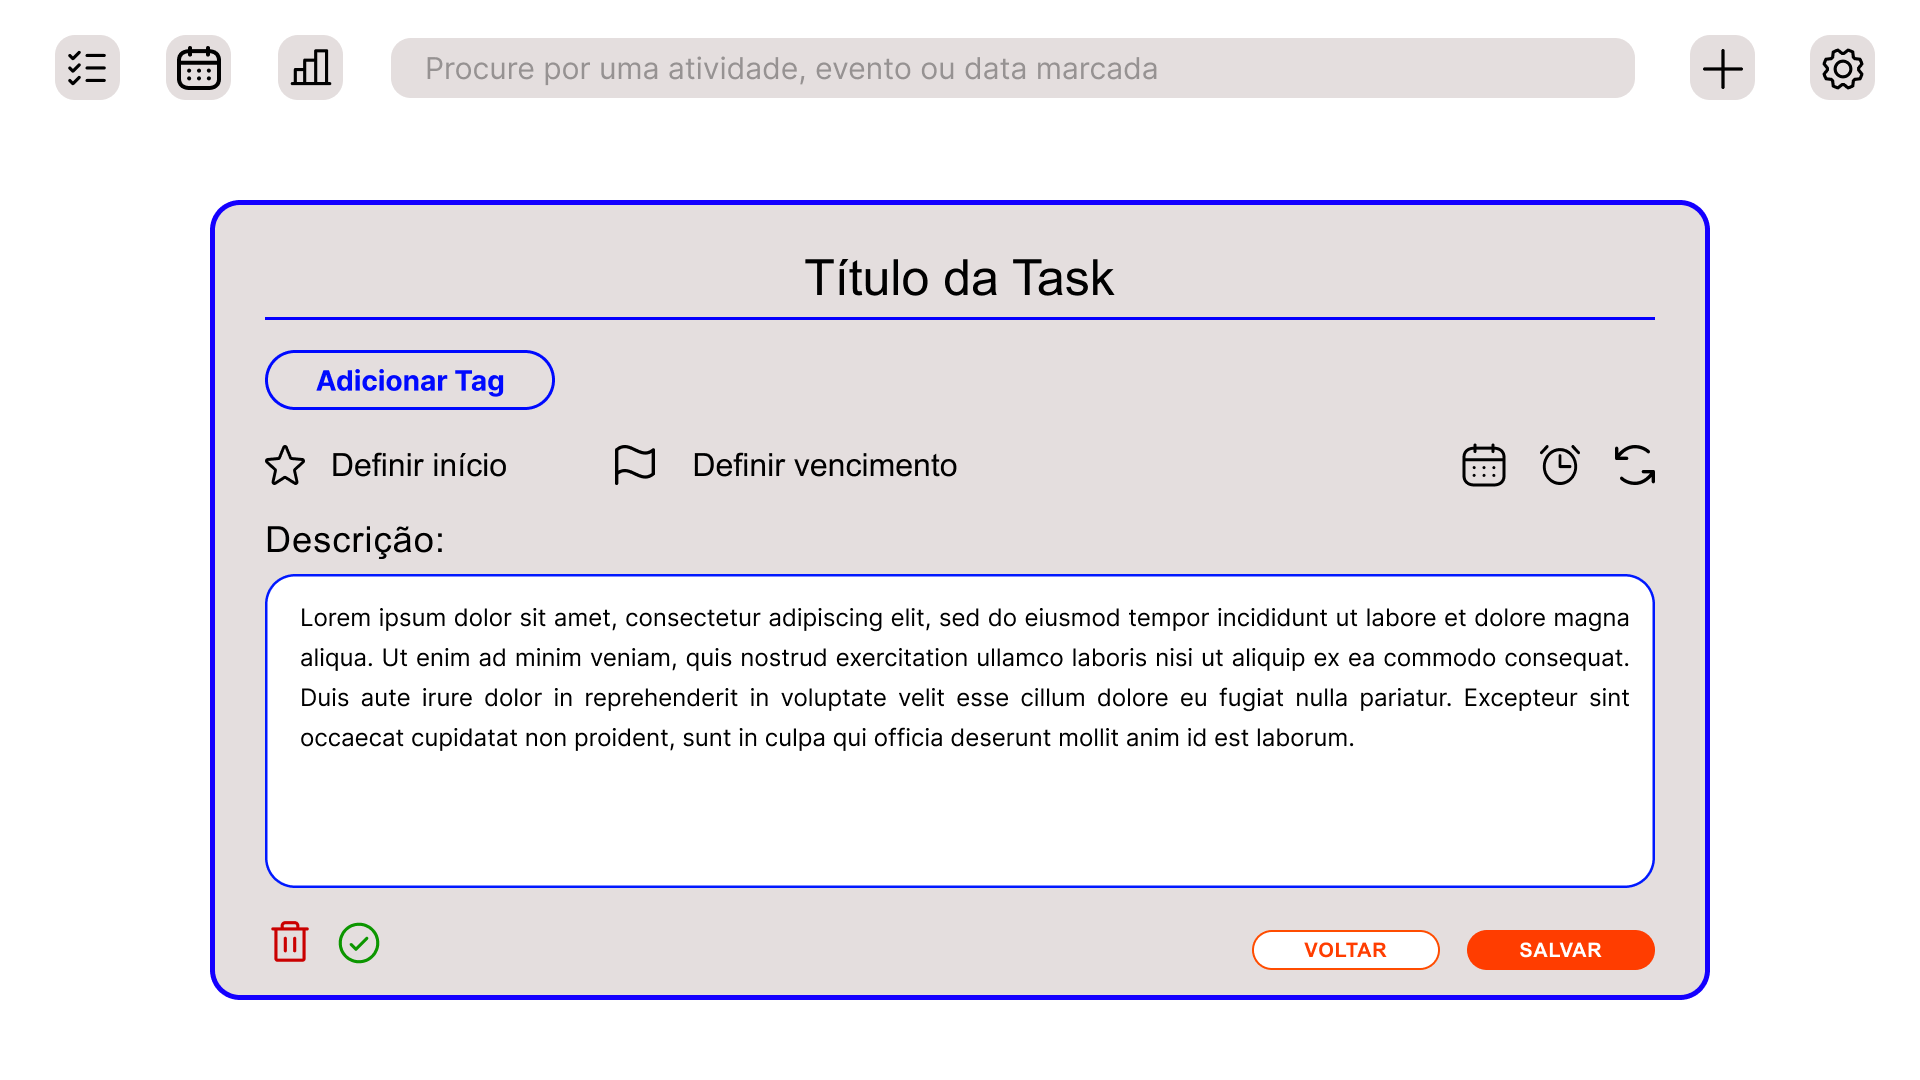
\includegraphics[scale=0.19]{prototypes/white/Add Task Panel Window.png}
		\caption{JPanel de Adição de Tasks - Modo Claro}
	\end{figure}
	\noindent Fonte: Os Autores.

	\item Tela de Edição de Tasks
	\begin{figure}[H]
		\centering
		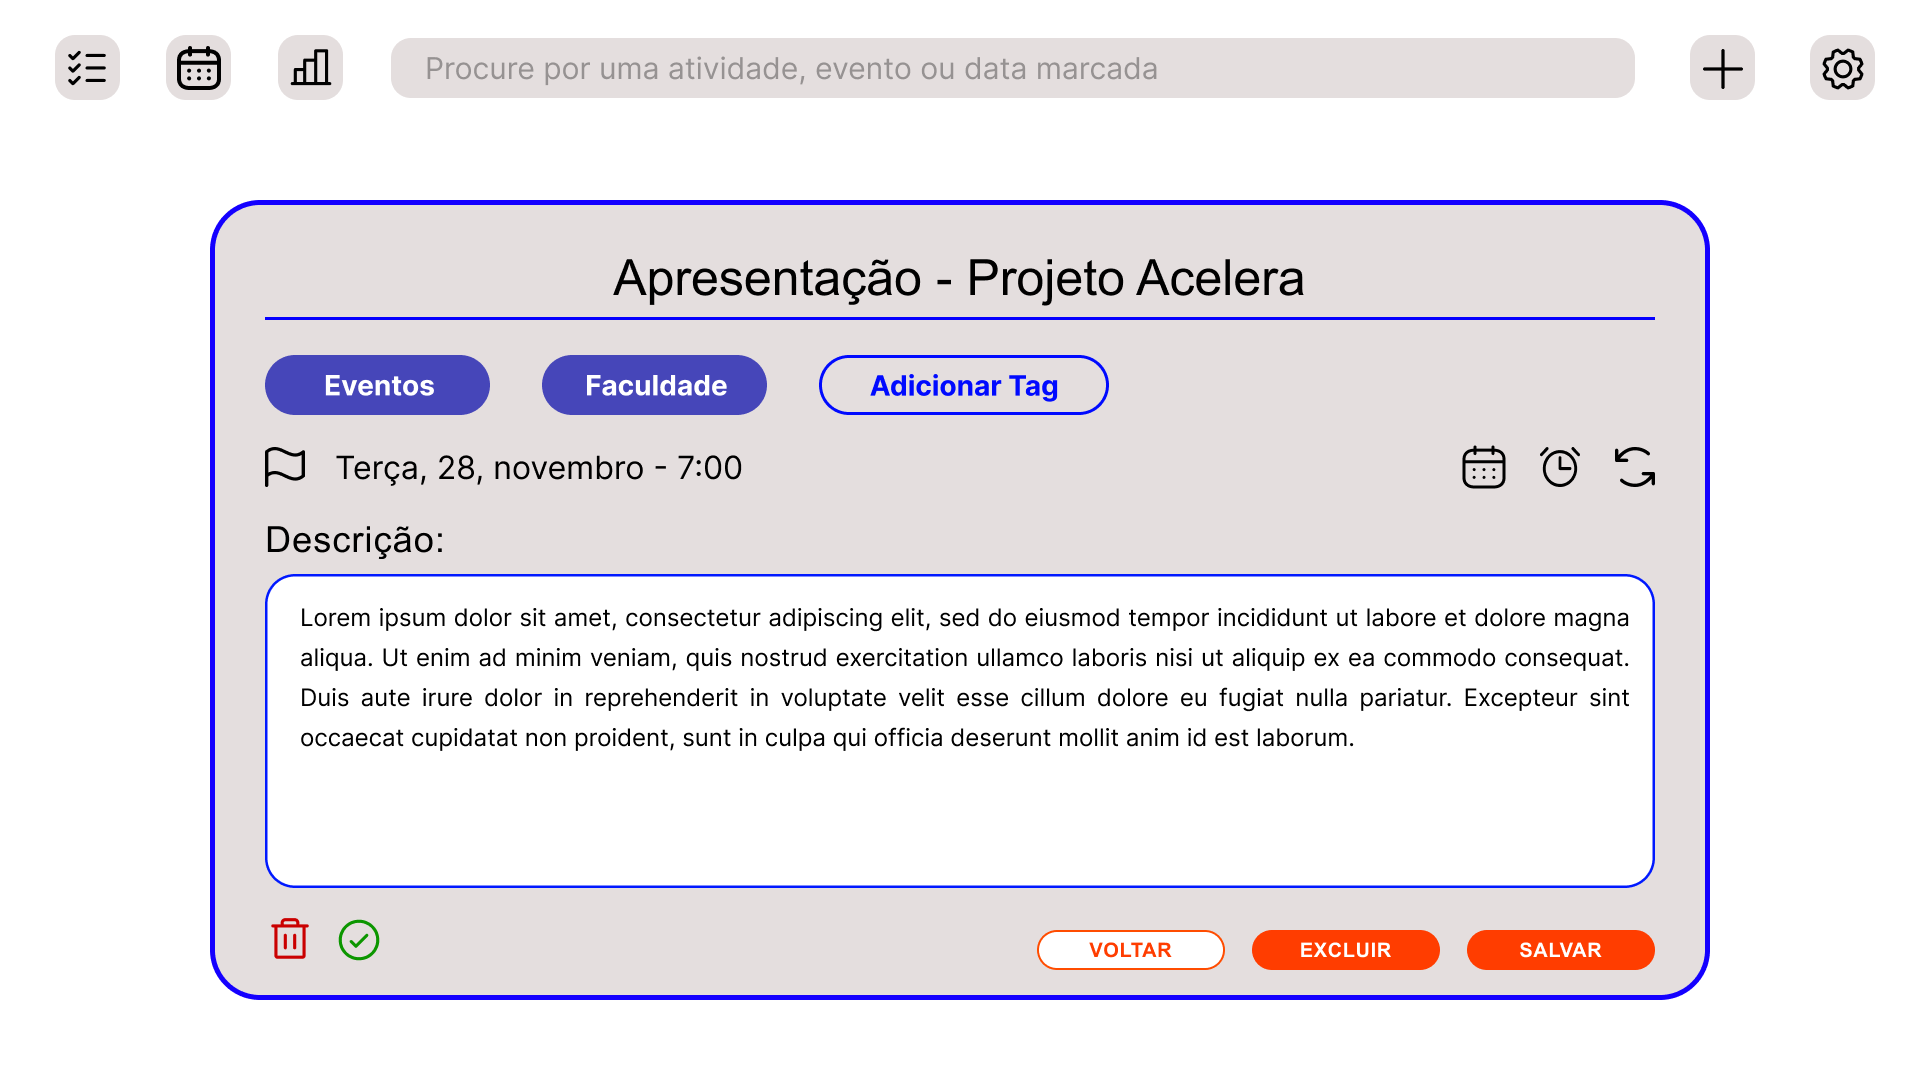
\includegraphics[scale=0.19]{prototypes/white/Edit Task Panel Window.png}
		\caption{JPanel de Edição de Tasks - Modo Claro}
	\end{figure}
	\noindent Fonte: Os Autores.
\end{itemize}	

\pagebreak
\subsubsection{Tema Escuro}
Telas com tema escuro são aquelas que apresentam cores mais escuras, como o preto, o cinza escuro, o azul escuro, entre outros. A ideia de um tema escuro 
é a de que o usuário possa utilizar o sistema em ambientes com iluminação mais fraca, como em ambientes internos, por exemplo.

\begin{itemize}
	\item Tema Principal
	\begin{figure}[H]
		\centering
		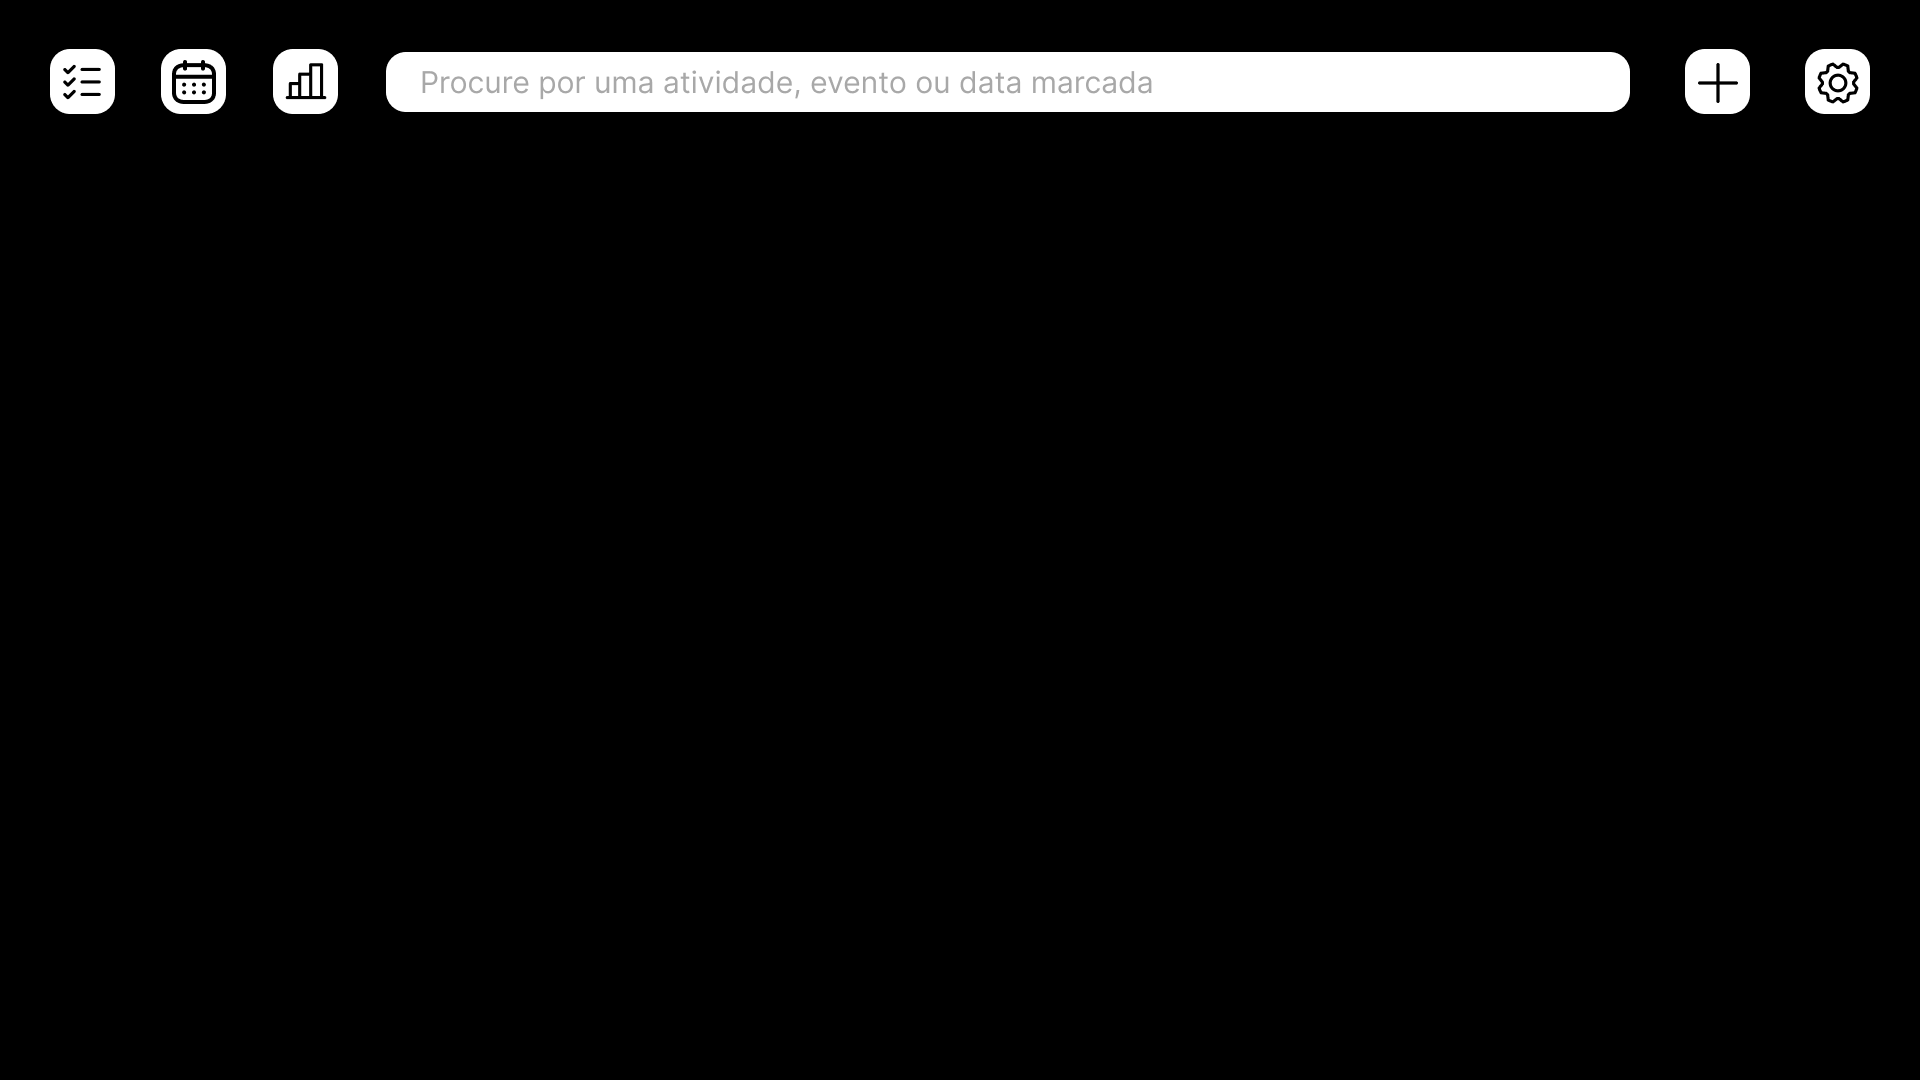
\includegraphics[scale=0.19]{prototypes/dark/Main Window.png}
		\caption{JFrame principal - Modo Escuro}
	\end{figure}
	\noindent Fonte: Os Autores.
	\item Calendário de Tasks
	\begin{figure}[H]
		\centering
		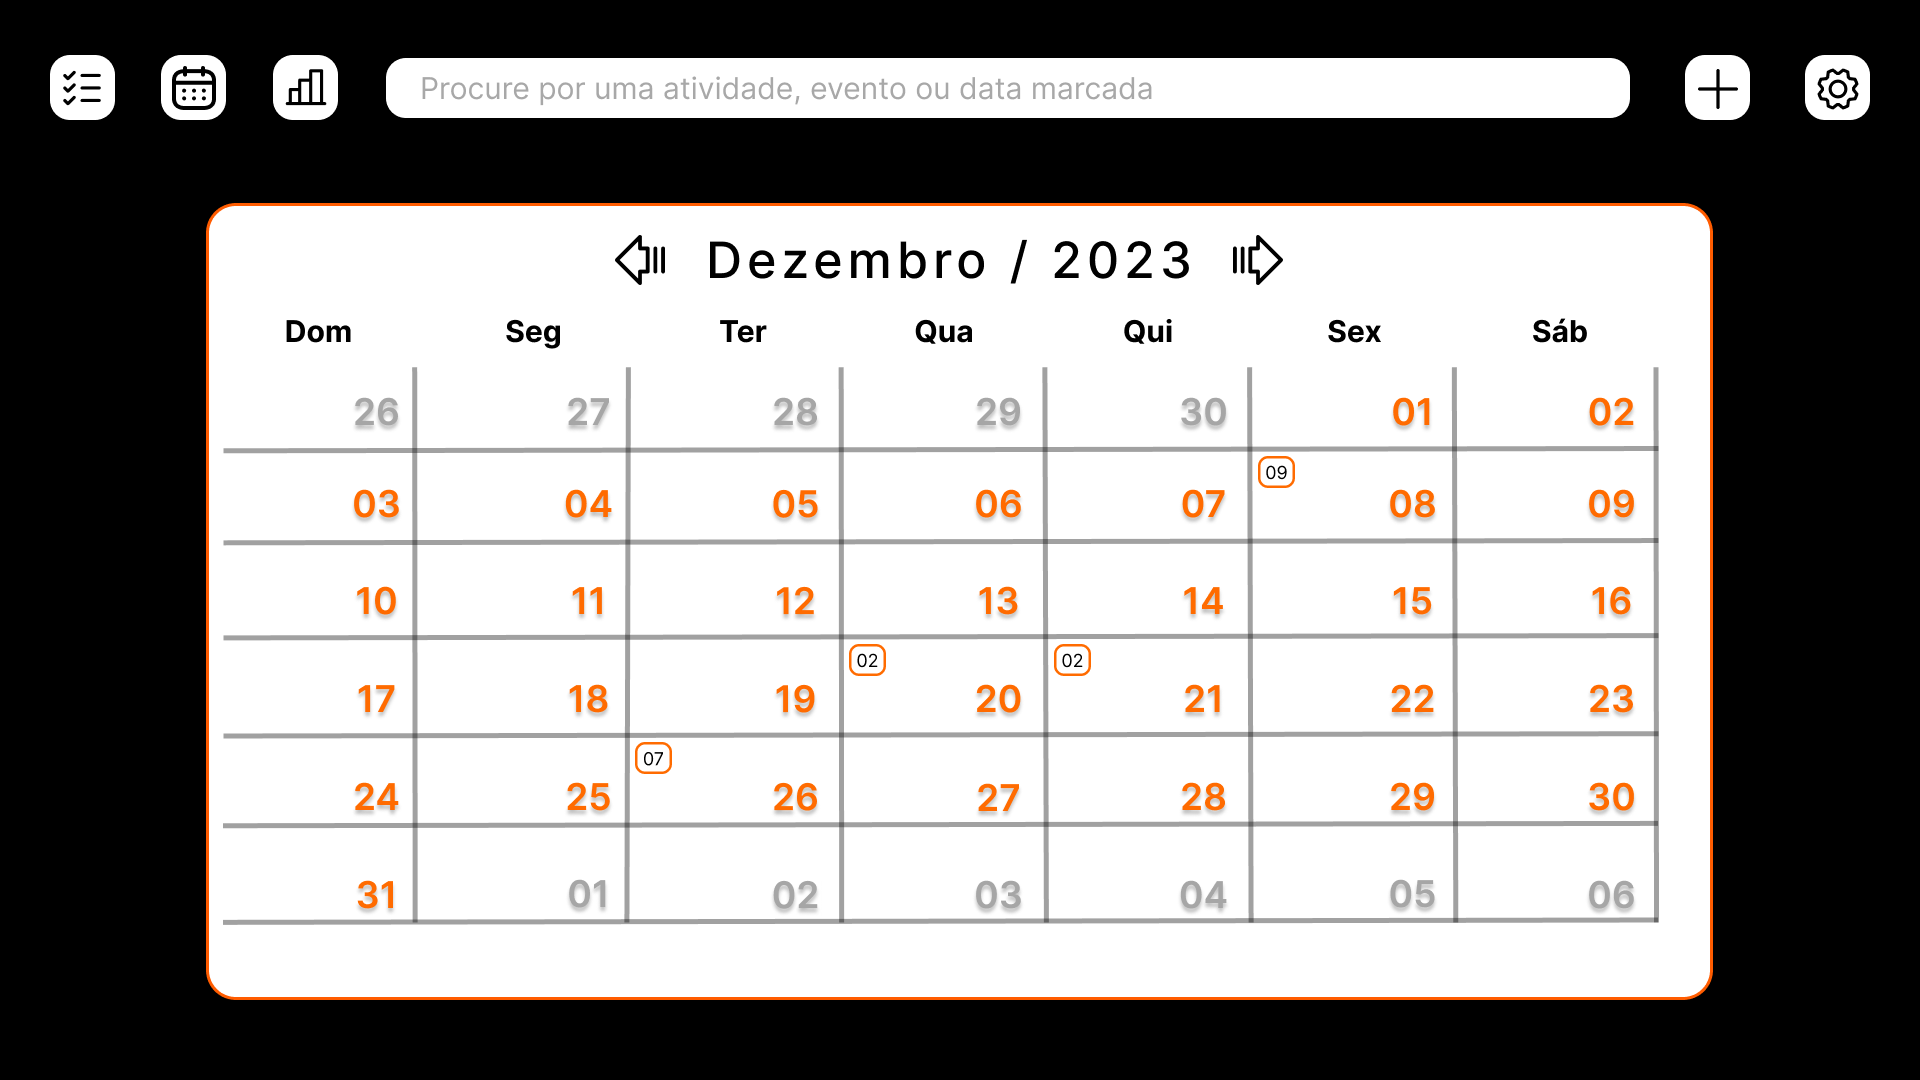
\includegraphics[scale=0.19]{prototypes/dark/Calendar Panel Window.png}
		\caption{JPanel Calendário - Modo Escuro}
	\end{figure}	
	\noindent Fonte: Os Autores.
	\pagebreak
	\item Estatísticas Gerais
	\begin{figure}[H]
		\centering
		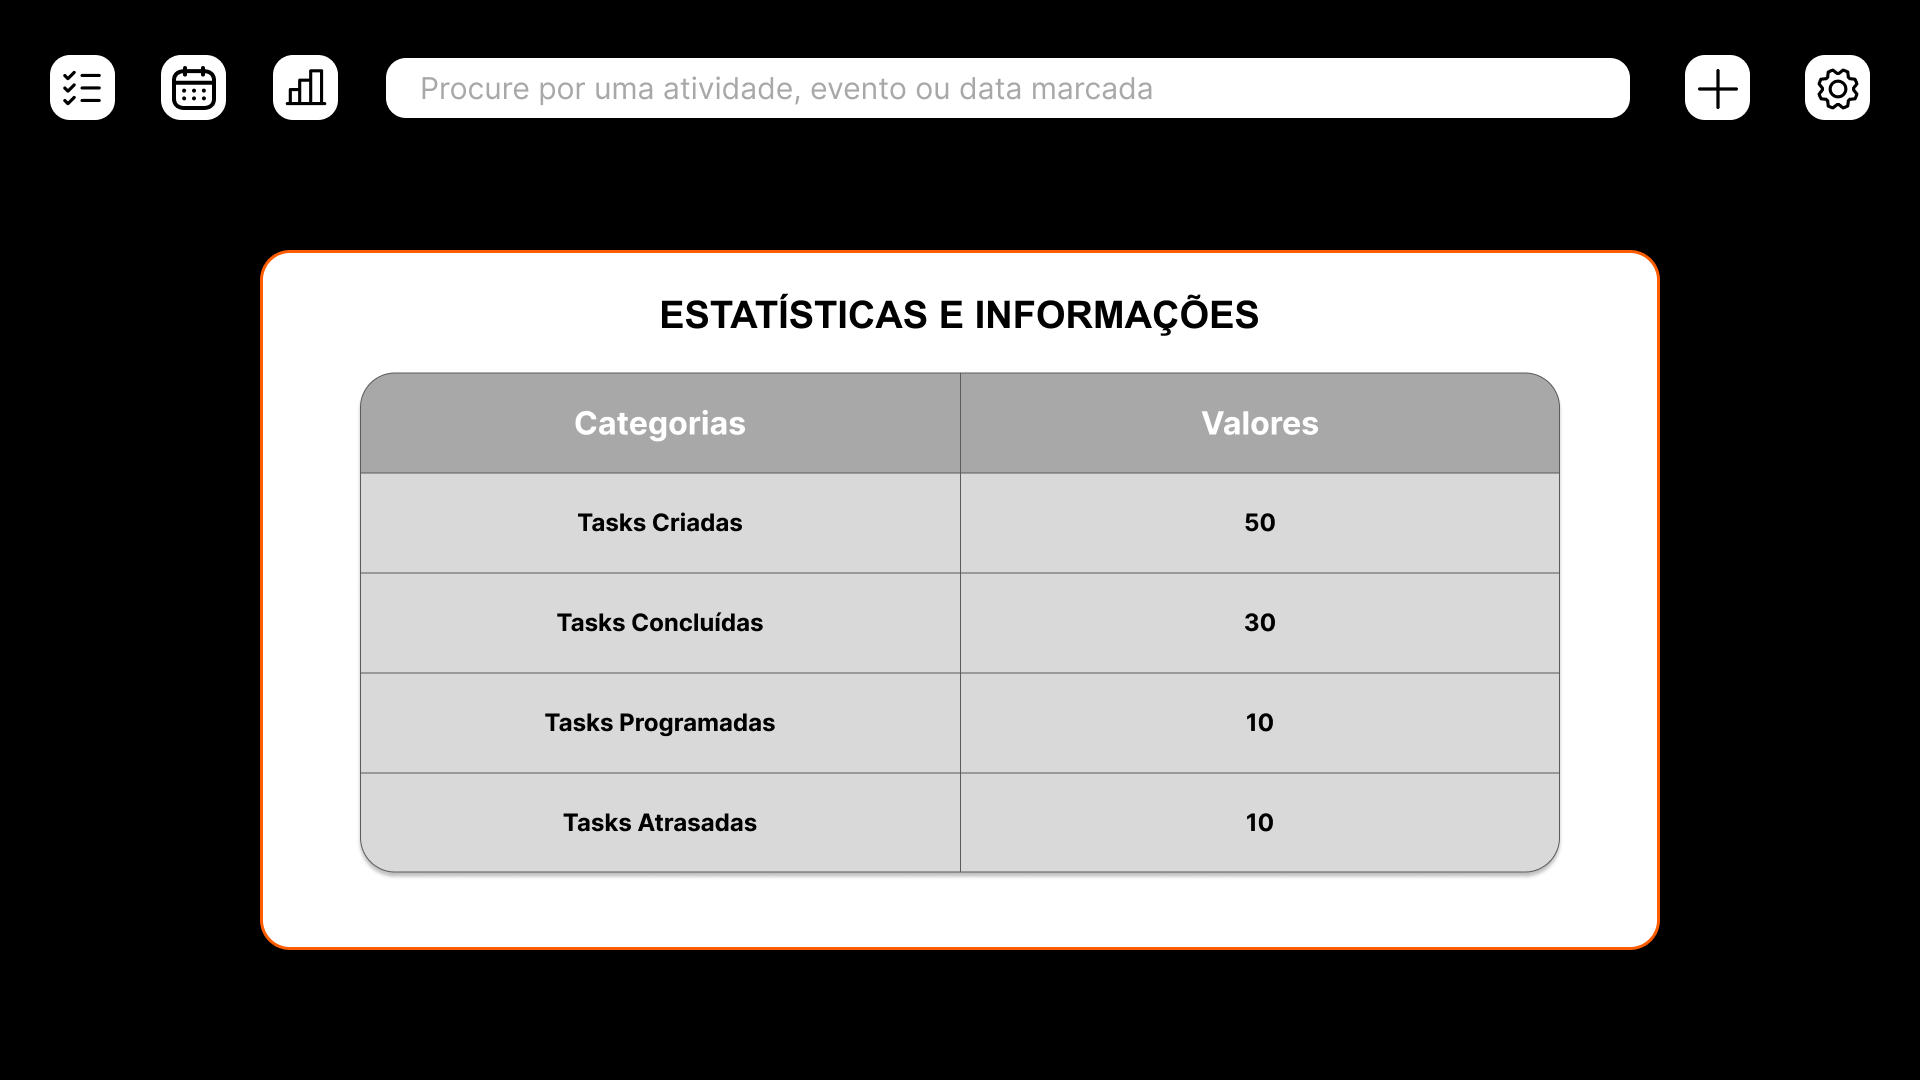
\includegraphics[scale=0.19]{prototypes/dark/Stats Panel Window.png}
		\caption{JPanel de Informações e Estatísticas - Modo Escuro}
	\end{figure}
	\noindent Fonte: Os Autores.
	\item Tela de Configuração
	\begin{figure}[H]
		\centering
		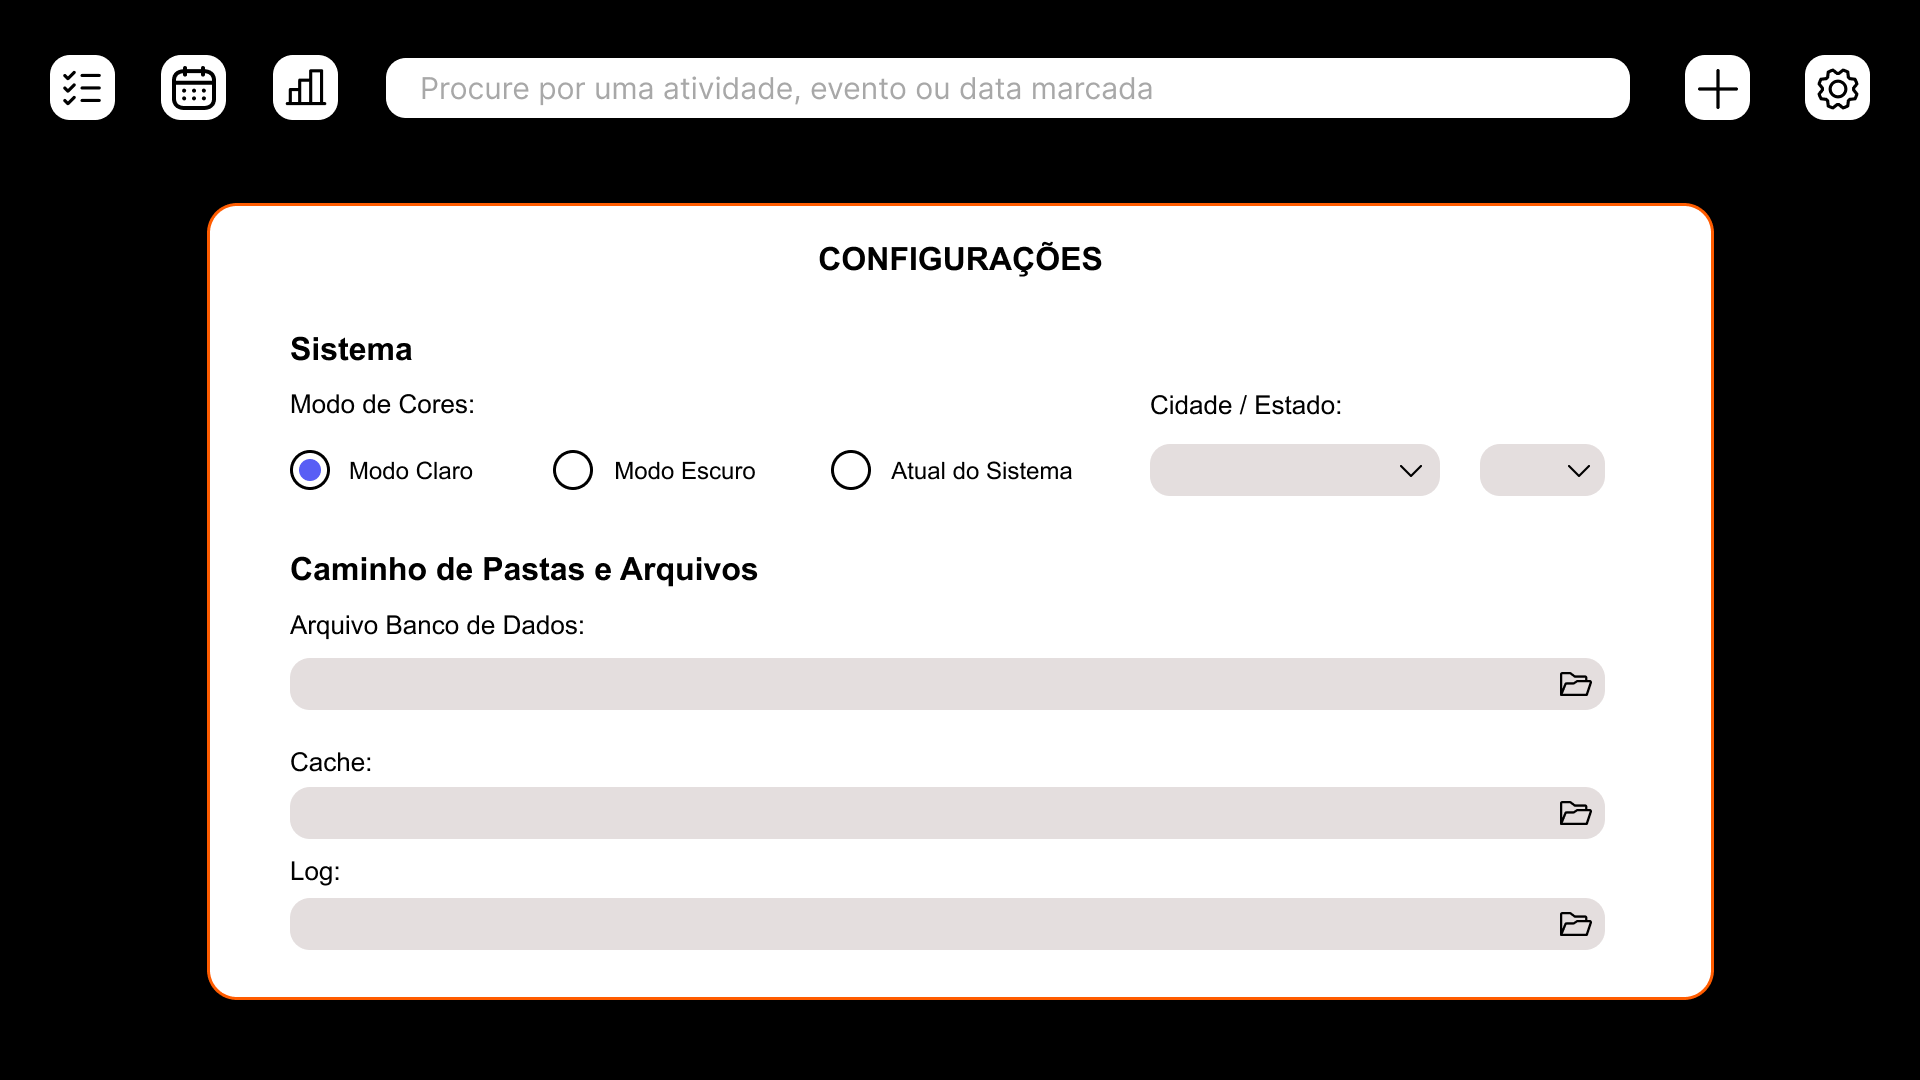
\includegraphics[scale=0.19]{prototypes/dark/Config Panel Window.png}
		\caption{JPanel de Configurações - Modo Escuro}
	\end{figure}
	\noindent Fonte: Os Autores.
	\pagebreak
	\item Tela de Adição de Tasks
	\begin{figure}[H]
		\centering
		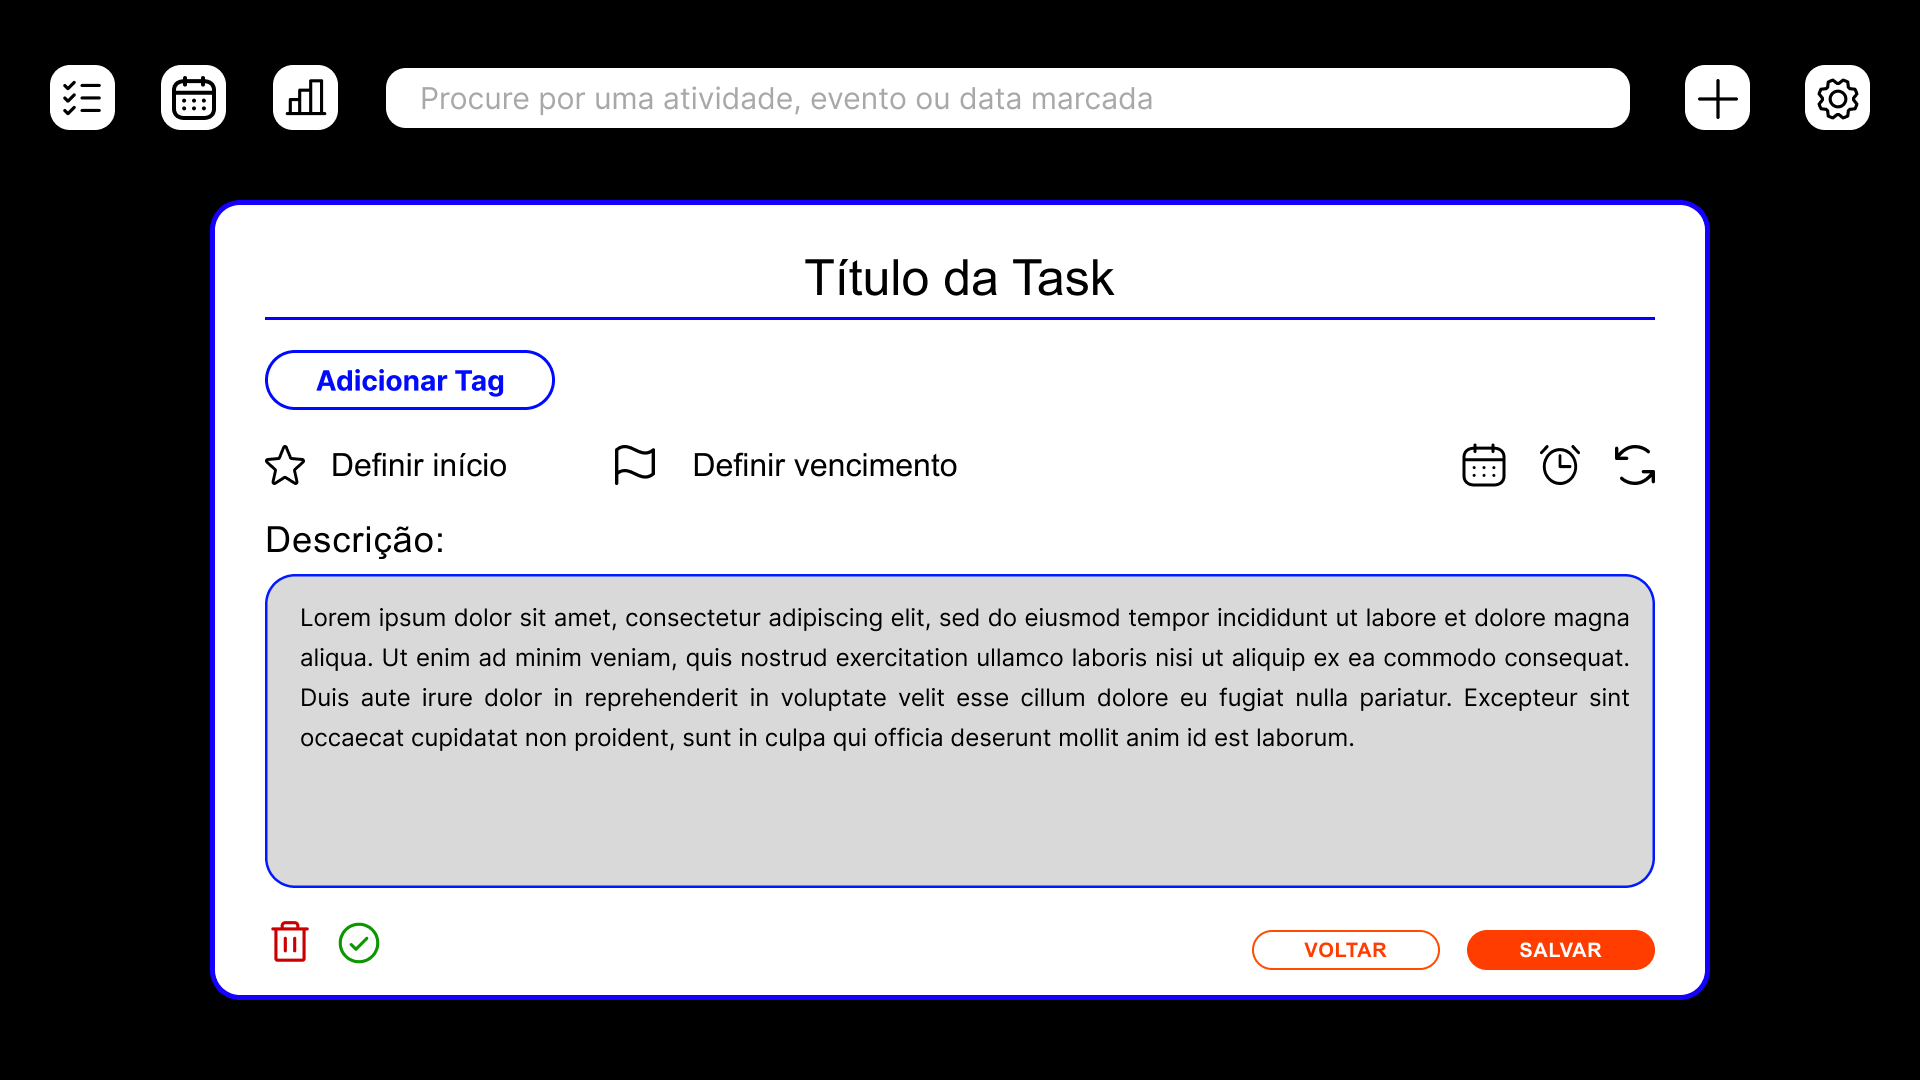
\includegraphics[scale=0.19]{prototypes/dark/Add Task Panel Window.png}
		\caption{JPanel de Adição de Tasks - Modo Escuro}
	\end{figure}
	\noindent Fonte: Os Autores.
	\item Tela de Edição de Tasks
	\begin{figure}[H]
		\centering
		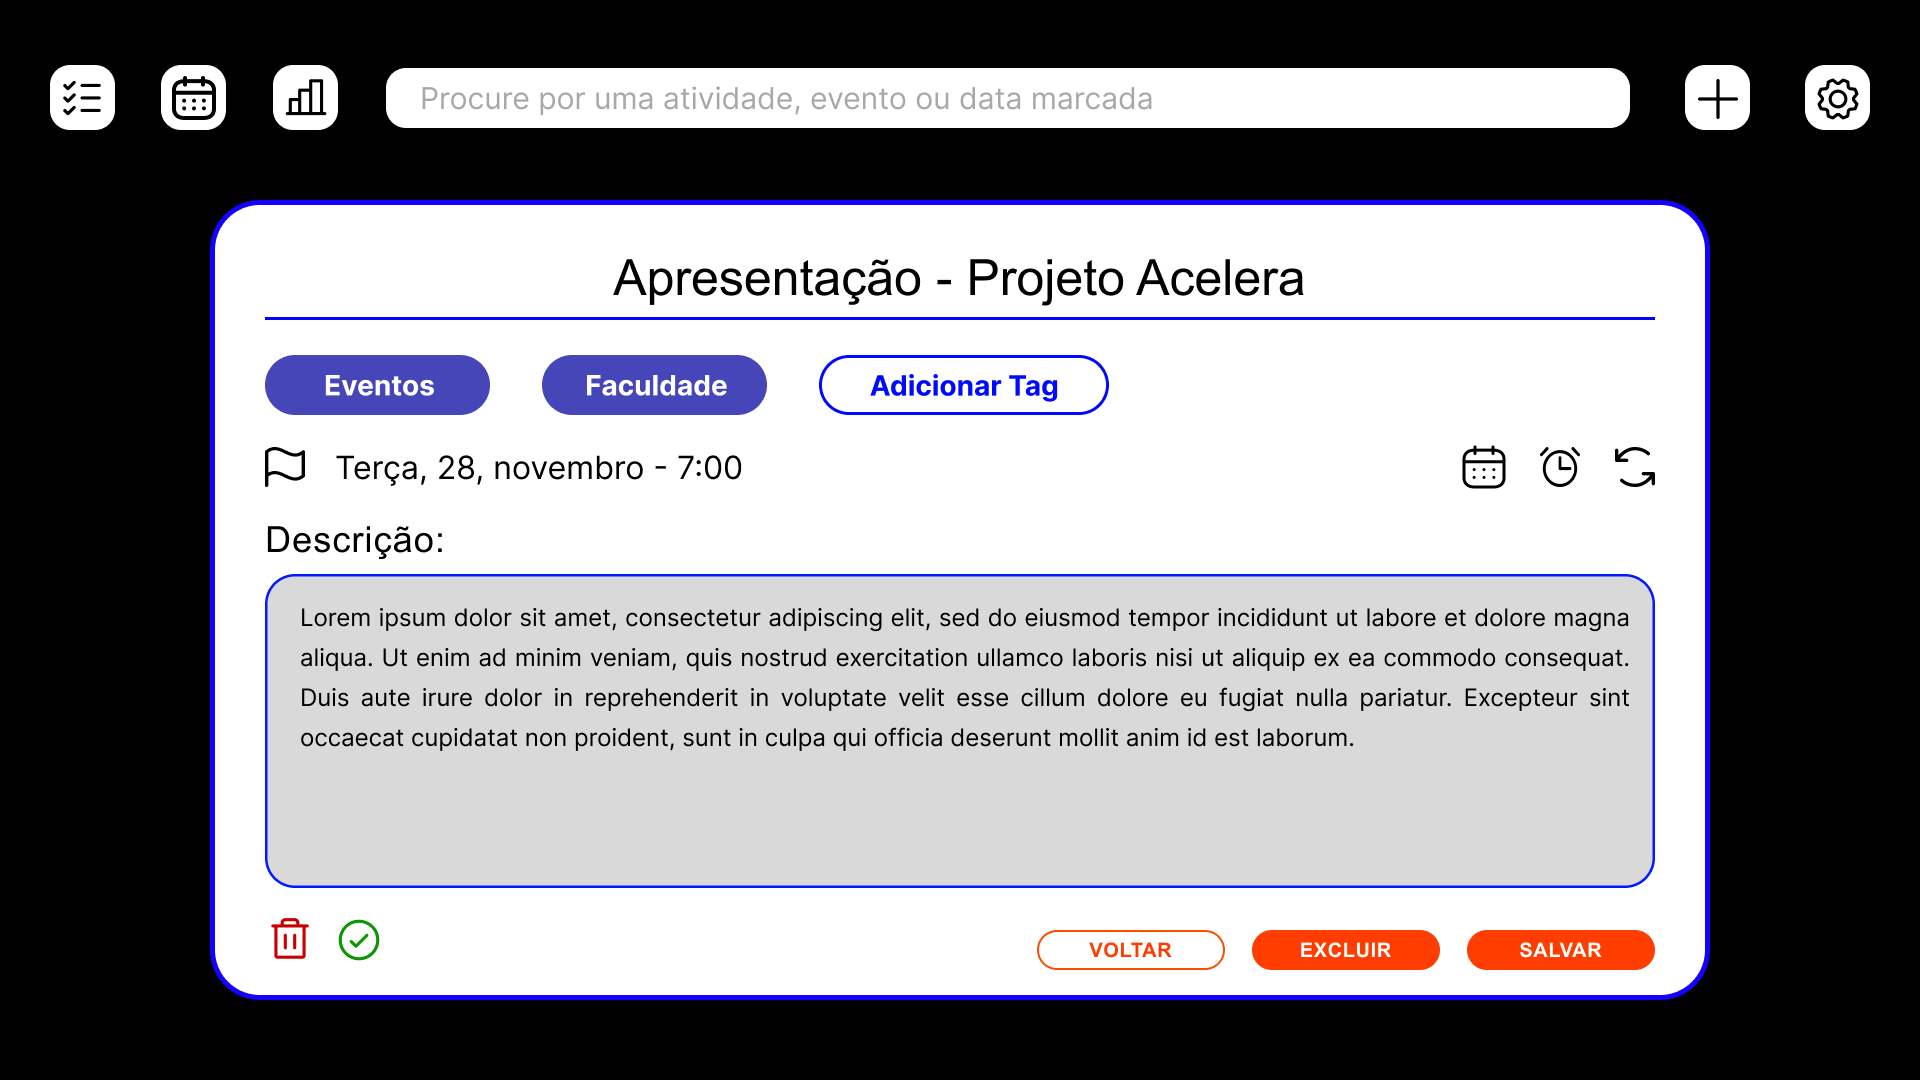
\includegraphics[scale=0.19]{prototypes/dark/Edit Task Panel Window.png}
		\caption{JPanel de Edição de Tasks - Modo Escuro}
	\end{figure}
	\noindent Fonte: Os Autores.
\end{itemize}

\pagebreak
A seguir, temos outros JFrames que servirão como modais, ou pequenas telas informativas e de confirmação de ações, que serão apresentadas sobre a 
tela principal, e que serão apresentadas em ambos os temas, claro e escuro.
\begin{itemize}
	\item Tela de Confirmação de Exclusão de Tasks
	\begin{figure}[H]
		\centering
		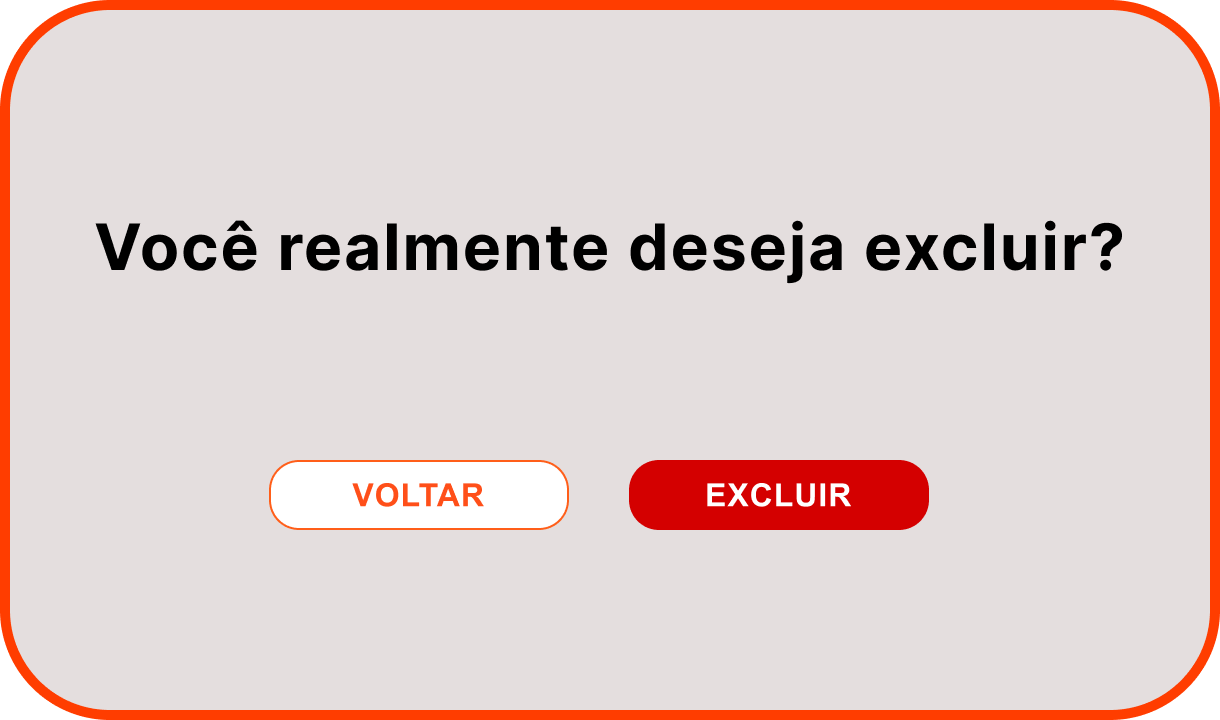
\includegraphics[scale=0.19]{prototypes/white/Modal Confirmation.png}
		\caption{JFrame de Confirmação de Exclusão de Tasks}
	\end{figure}
	\noindent Fonte: Os Autores.
	\item Tela de Criação de Tags
	\begin{figure}[H]
		\centering
		\includegraphics[scale=0.19]{prototypes/white/Add Tag.png}
		\caption{JFrame de Criação de Tags}
	\end{figure}
	\noindent Fonte: Os Autores.
	\item Tela de Sobre (Equipe e Sistema)
	\begin{figure}[H]
		\centering
		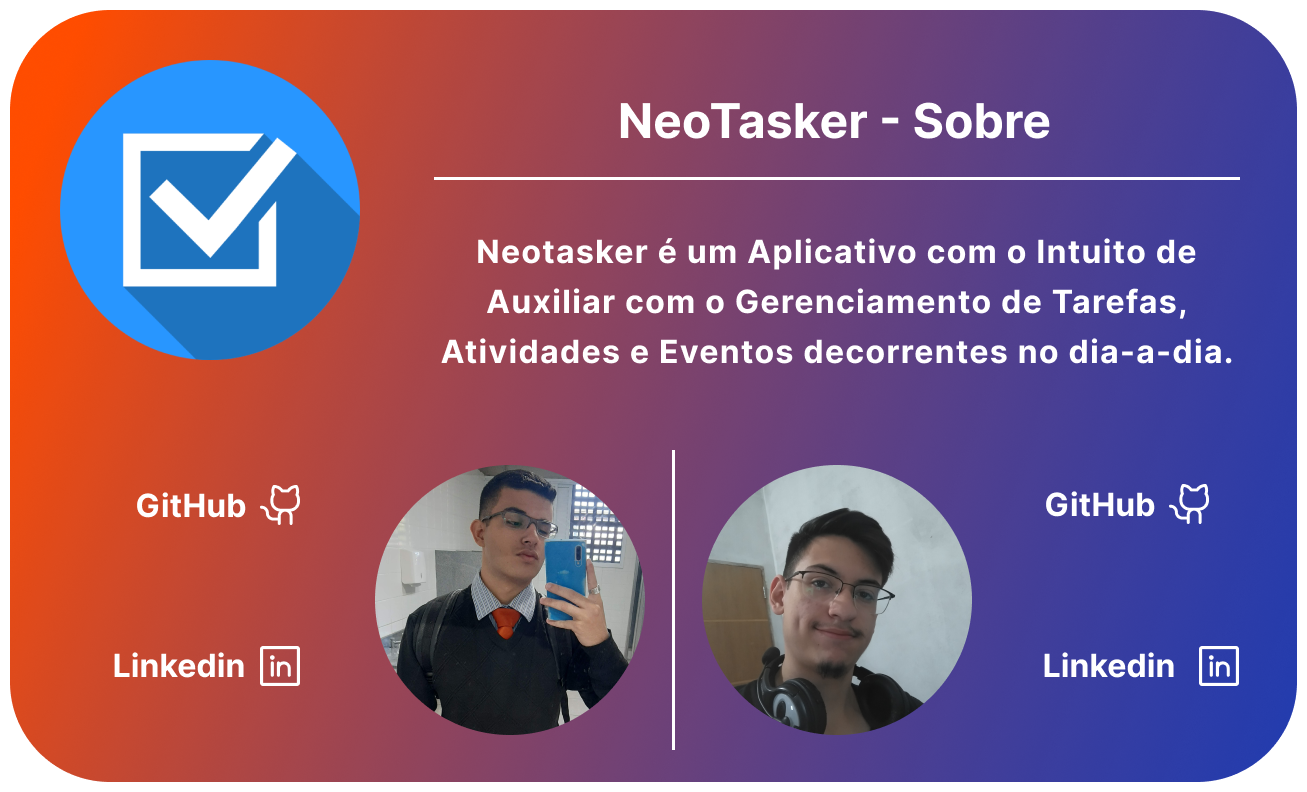
\includegraphics[scale=0.19]{prototypes/white/About Us Panel Window.png}
		\caption{JFrame de Sobre (Equipe e Sistema)}
	\end{figure}
	\noindent Fonte: Os Autores.
\end{itemize}


% --- Segment: Development ---
\pagebreak
\section{Desenvolvimento}
% --- Segment: Database ---
\subsection{Banco de Dados}
Banco de Dados é um sistema capaz de adicionar uma coleção de registros em um repositório computacional. Basicamente, o arquivamento de 
registros em um armário a fim de registrar dados de pessoas, física ou jurídica, no entanto de maneira computadorizada, é classificada 
como um Banco de Dados. Quando se necessita armazenar um fluxo de informações e futuramente recuperá-las, buscando-as e consultando-as 
no sistema, opta-se pelo uso desta tecnologia. (DATE, 2004; ALVES, 2021).

No Banco de Dados, pode ser feita uma manipulação geral através de ações independente qual seja. Adicionando, alterando, consultando 
ou anulando algum dado, o gerenciamento é feito. As informações que podem, ou não, ser inseridas no banco podem ser qualquer uma que 
dê característica há quem ela pertence, ou seja, significativa para o seu indivíduo detentor. Os dados armazenados são modelados em 
linhas e colunas, de modo que as ações de manipulação possam ser feitas facilmente. (ELMASRI et al., 2005; DATE, 2004).

Ainda hoje, organizações dos mais diferentes feitios utilizam papéis para agregar registros de pessoas e arquivos gerais. Mas em cenários
de muitas pessoas em uma localidade, uma quantidade exacerbada de dados se encontra em trânsito, principalmente pela alta requisição deles. 
Por isso, faz-se viável a utilização de um sistema computacional para armazenar todo tipo de informação. O uso de um Banco de Dados nas 
organizações é comum na sociedade atual, já que se tornou componente essencial na sociedade moderno. Com as funcionalidades presentes em 
uma base de dados, podem ser inseridas essas grandes cargas de informações, tornando assim o processo automatizado, confiável e eficiente. 
A exemplo, uma instituição educacional possui diversos dados de alunos, professores e até mesmo funcionários, necessitando um sistema 
eletrônico para gerenciar toda essa carga de registros; Através do banco dessa instituição, pode-se, por exemplo, saber notas e menções 
de alunos e saber qual o conteúdo qual professor está dando para cada turma à qual ele foi designado. (ALVES, 2021).

Usar uma base de dados torna o conjunto de todo o sistema automatizado e ágil no fluxo de informações, promovendo o armazenamento 
de dados sobre contas, negociações, documentos, pessoas etc. A procura e acesso ao banco de dados, daqueles usuários que forem detentores 
da permissão, será feita, assim será possível manipular os registros. (FILHO; IOCHPE, 2001).

\subsubsection{Banco de Dados Relacional}
A maneira de representar dados em um banco de relações demanda o uso de tabelas com nome próprio para identificar a entidade, que é 
algo do mundo real que possui existência independente. Já os atributos, também chamadas de colunas ou campo de seleção, recebem os 
dados correspondentes as entidades nas linhas não ordenadas. (TONSIG, 2006; MACÁRIO; BALDO, 2005). 

\subsubsection{Relacionamentos}
O envio de chaves primárias como chaves estrangeiras para outras tabelas é o que estabelece a relação entre tabelas. O relacionamento 
existente entre cada par de tabelas pode ser classificado em diferentes tipos, são eles:
\begin{itemize}
	\item\textbf{um para muitos (1:N):} quando a tabela A, pode possuir e estar uma ou mais vezes presentes em um cenário, já a tabela B está presente somente uma 
	única vez no cenário a cada momento. Neste caso, necessita-se que o atributo que identifica o registro da tabela B vá como atributo estrangeiro para 
	a tabela A; (RANGEL, 2004; TONSIG, 2006).
	\item\textbf{um para um (1:1):} neste caso, as duas tabelas se relacionam uma com a outra somente uma vez a cada momento 
	no cenário da relação; (RANGEL, 2004; TONSIG, 2006).
	\item\textbf{muitos para muitos (N:M):} neste exemplo, as tabelas A e B estão presentes uma ou mais vezes em um cenário. 
	A particularidade dessa relação é que as chaves primárias das tabelas A e B vão para uma terceira tabela, a tabela C de relacionamento, 
	onde também haverá o atributo identificador. (RANGEL, 2004; TONSIG, 2006).
\end{itemize}

\subsubsection{Sistema de Gerenciamento de Banco de Dados}
O conjunto de ferramentas e programas que dá suporte a realização das ações, citadas anteriormente, em uma Base de Dados, é conhecido como 
Sistema Gerenciador de Banco de Dados (SGBD). Um SGBD é destinado à definição, construção e manipulação do banco. (TONSIG, 2006; FILHO; IOCHPE, 2001). 

Os vocábulos Sistema de Banco de Dados (SBD) e Sistema Gerenciador de Banco de Dados (SGBD) são expressos no mesmo sentido, dando mesmo 
significado, no entanto cada um representa definições distintas. Portanto, quando um SGBD é integrado ao Bando de Dados (BD), junto aos 
programas de aplicação, temos um SBD. Para que alterações, consultas, inserções e exclusões sejam executadas, uma sintaxe é fundamental 
para que o SGBD possa interpretar e manipular os dados em um Banco. Atualmente, a maioria dos sistemas para gerenciar o banco utiliza a 
linguagem \textit{Structured Query Language} (SQL), considerada uma linguagem de consulta, antes conhecida 
como \textit{Structured English Query Language} (SEQUEL). Entretanto, outros softwares SGBDs utilizam a própria linguagem de 
consulta para sua Base de Dados. Os SGBDs mais usados e 
conhecidos atualmente são Interbase, SQL Server, Oracle, que é a líder no mercado de banco de dados relacionais, 
MySQL e SQlite3, sendo este último o escolhido para o desenvolvimento deste projeto. (TONSIG, 2006; DATE, 2004; MACÁRIO; BALDO, 2005). 

Para auxiliar no desenvolvimento das tabelas do banco de dados, ainda foi utilizado o suporte de um ORM\footnote{
	\textit{Object-Relational Mapping} (ORM), em português, Mapeamento Objeto-Relacional, é uma técnica para aproximar o paradigma de desenvolvimento de aplicações orientadas a objetos ao paradigma do banco de dados relacional. O uso da técnica de ORMs é realizado através de um ORM que geralmente é a biblioteca ou \textit{framework} que ajuda no mapeamento e uso do banco de dados.
}, através da biblioteca Hibernate ORM, que permite a criação de tabelas e relacionamentos entre elas, além de facilitar a manipulação dos dados. Abaixo, segue o diagrama de entidade e relacionamento do banco de dados do sistema:
\begin{figure}[H]
	\centering
	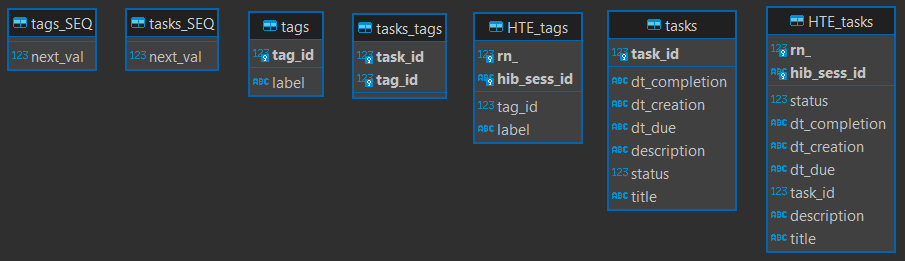
\includegraphics[scale=0.80]{database/database-diagram.png}
	\caption{Diagrama de Entidade e Relacionamento do Banco de Dados}
\end{figure}
\noindent Fonte: Os Autores.

% --- Segment: Back-End ---
\subsection{Java}
Java é uma linguagem de programação desenvolvida pela empresa Sun Microsystems, em 1995. Atualmente, quem possui os direitos da 
linguagem é a Oracle Corporation. A linguagem Java é uma linguagem de programação de propósito geral, ou seja, pode ser utilizada 
para desenvolver qualquer tipo de aplicação, desde aplicações desktop até aplicações web, includindo aplicações robustas e comerciais. (ARNOLD et al., 2005)

As possibilidades com Java são diversas, o que a configura atualmente, de acordo com o rankings da TIOBE de novembro de 2023, como a 4ª linguagem de programação
mais utilizada no mundo. No entanto, de acordo com dados do próprio TIOBE, Java ja esteve na lidenrança do ranking, sendo a linguagem mais utilizada do mundo
por um período de aproximadamente entre 15 e 20 anos. (TIOBE, 2023)

\subsubsection{Breve Histórico}
Java começou a surgir com o Projeto Green, em 1991, na Sun Microsystems, com James Gosling, sendo ele o nome mais relacionado a Java dentre as pesquisas 
sobre o tema. O Projeto Green consistia no desenvolvimento de tecnologias modernas de software para dispositivos eletrônicos. Além disso, a ferramenta
em desevolvimento precisava ser compatível com a necesssidade de quem a fosse usar, de modo que seu código fosse compacto e com arquitetura neutra. (JAVA; SOARES INDRUSIAK, 1996)

O objetivo incial foi comprido, no entanto, Java começou com uma participação de mercado pequena. 

Coincidentimente, no mesmo período o início da Wolrd Wide Web (WWW) começava a surgir. Como uma oportunidade de negócio a vista, os desevoldores da Sun
Microsystems, optaram por adaptar a tecnologia que possíam no momento para o ambiente da web, permitindo o desenvolvimento de aplicações e programas para web.
Logo, Java se torou um sucesso, principalmente no momento de lançamento do HotJava, o primeiro navegador web com suporte para a linguagem recém criada. (JAVA; SOARES INDRUSIAK, 1996)

Abaixo segue características fundamentais no entendimento da linguagem Java:
\begin{itemize}
	\item \textbf{Orientação a Objetos:} Java é uma linguagem de programação orientada a objetos, o que permite seu fácil uso e abstração do mundo real em diferentes necessidades; (CLARO; BOSCO; SOBRAL, 2008)
	\item \textbf{Multiplataforma:} Java é uma linguagem de programação multiplataforma, ou seja, pode ser executada em qualquer sistema operacional, desde que possua uma máquina virtual Java (JVM) instalada; (CLARO; BOSCO; SOBRAL, 2008)
	\item \textbf{Gestão de Processos} Java é uma linguagem de programação segura, ou seja, possui uma série de mecanismos que garantem a segurança de suas aplicações, como por exemplo, o uso de um \textit{Garbage Collector}, 
	que é um coletor de lixo que gerencia a memória da aplicação, evitando o uso de memória desnecessária e vazamentos de memória; (CLARO; BOSCO; SOBRAL, 2008)
	\item \textbf{Portável:} O código desenvolvido em Java, após o seu estado de interpretação de código, o chamado \textit{bytecode}\footnote{
		Código intermediáio gerado após a intepretação da IDE. Este não é o código final executável no sistema.
	}, com auxílio da JVM, é capaz de ser compilado em qualquer sistema operacional. (CLARO; BOSCO; SOBRAL, 2008)
\end{itemize}

\subsubsection{Java Development Kit}
O Java Development Kit, ou JDK (Kit de Desenvolvimento Java, em português), é um conjunto de ferramentas para desenvolvimento de aplicações em Java. Este pacote oferece ferramentas 
de compilação de código e interpretação, além de utilitários como biblitecas nativas da linguagem para auxiliar na implementação do código-fonte em Java. Dentre as principais ferramentas do JDK, temos:
\begin{itemize}
	\item \textbf{javac:} Compilador Java, responsável por transformar o código-fonte em Java em \textit{bytecode}, ou seja, o código intermediário que será interpretado pela JVM; (CLARO; BOSCO; SOBRAL, 2008)
	\item \textbf{java:} Interpretador Java, responsável por interpretar o \textit{bytecode} gerado pelo compilador Java, transformando-o em código de máquina, ou seja, o código final executável no sistema; (CLARO; BOSCO; SOBRAL, 2008)
	\item \textbf{javadoc:} Gerador de documentação Java, responsável por gerar a documentação do código-fonte em Java, através de comentários especiais no código; (CLARO; BOSCO; SOBRAL, 2008)
	\item \textbf{appletviewer:} Visualizador de Applets Java, responsável por executar applets Java, que são pequenas aplicações desenvolvidas em Java, que são executadas em navegadores web; (CLARO; BOSCO; SOBRAL, 2008)
	\item \textbf{javafxpackager:} Ferramenta para empacotamento de aplicações JavaFX, responsável por empacotar aplicações desenvolvidas em JavaFX, que é uma biblioteca gráfica para desenvolvimento de interfaces gráficas em Java; e(CLARO; BOSCO; SOBRAL, 2008)
	\item \textbf{jar:} Ferramenta para empacotamento de aplicações Java, responsável por empacotar aplicações desenvolvidas em Java, que são executadas em linha de comando; (CLARO; BOSCO; SOBRAL, 2008)
\end{itemize}

Atualmente o JDK está sendo implementado utilizando das versões 17 ou 21 do pacote, isto é, pois há uma transição entre versões. As informações entre versões e demais opções de donwloads 
podem ser encontradas no site oficial da Oracle, no link https://www.oracle.com/java/technologies/downloads/ .



\subsubsection{Orientação a Objetos}
Abordar Java ou quaisquer outras linguagens que utilizam da Orientação a Objetos como paradigma, se faz necesário que entendamos, de forma geral,
o que é a Orientação a Objetos de fato.

Em um contexto geral da década de 1980 e 1990, onde a manipulação de dados complexos e entidades/personagens do mundo real cresceu de forma exponente,
a dificuldade em reutilizar e implantar sistemas que possuíam uma grande quantidade de dados e informações, se tornou um problema. Logo, o paradigma do momento 
da programação estruturada, não era mais suficiente para atender a demanda de sistemas que necessitavam de uma maior organização e reutilização de código 
para replicar em diferentes realidades e ambientes. (CLARO; BOSCO; SOBRAL, [s.d.])

Como solução, um conceito de programação onde a abstração de dados permite a proximidade com o mundo real, de forma quase 100\% fidedignas a realidade foi desenvolvido.
A Orientação a Objetos, ou \textit{Object Oriented Programming} OOP, em inglês, é um paradigma de programação - desenvolvido na década de 1960, no entanto aplicado somente
porteriormente nos anos 1990 - que permite a criação de estruturas de dados de forma tais dados possam ser reaproveitados em diferentes 
ambiente, ocasiões, fluxos de negócios e domínio de mercado. A ideia é justamente a compatibilidade e reutilização de código,
através de técnicas como uso de classes, métodos, objetos, herança, polimorfismo, encapsulamento, entre outros. (CLARO; BOSCO; SOBRAL, [s.d.])

\subsubsection{EXPLICAR COMO APLICOU}
% COMO USOU A FERRAMENTA JAVA e POO PARA DESENVOLVER O BACK-END DO SISTEMA

% --- Segment: Front-End ---
\subsection{Java Swing}

\subsubsection{EXPLICAR COMO APLICOU}
% COMO USOU A FERRAMENTA JAVA SWING PARA DESENVOLVER O FRONT-END DO SISTEMA

\subsection{Abstract Window Toolkit - AWT}

\subsubsection{EXPLICAR COMO APLICOU}
% COMO USOU A FERRAMENTA JAVA AWT PARA DESENVOLVER O FRONT-END DO SISTEMA

% --- Segment: Bibs ---
\subsection{Outras Bibliotecas Utilizadas}
\subsubsection{Maven Assembly Plugin}
\subsubsection{SQlite3 JDBC Driver}
\subsubsection{Hibernate ORM + Community Dialects}
\subsubsection{JSoup}
\subsubsection{Google Gson}
\subsubsection{MigLayout}
\subsubsection{Formdev FlatLaf + IntelliJ Themes}

\subsection{Ferramentas}
O desenvolvimento do sistema foi feito em dois sistemas operacionais diferentes, sendo eles Window 11 e Arch Linux, logo, algumas ferramentas 
de codificação foram utilizadas em ambos os sistemas, mas pela diferença de plataformas, uma gama maior de softwares foi necessário. Abaixo, segue 
as informações de cada ferramenta utilizada no desenvolvimento do sistema, além de qual plataforma foi executado.

Dentre as ferramentas de desenvolvimento do código, temos:
\subsubsection{Visual Studio Code}
O Visual Studio Code é um editor de código-fonte, sua execução acontece a partir do acesso em seu atalho na área de trabalho do computador. 
Ele é executado em Windows, Linux e macOS. Além de forma nativa ele dispor de opções de tipo de arquivos, como arquivos .html, .php, .css etc, 
você pode baixar extensões que melhoram a gama de linguagens suportadas, a partir da biblioteca inserida no software. Outras extensões tratam da 
usabilidade do sistema, a partir de conexões com outras aplicações e atalhos na interface. Em resumo, as extensões buscam melhorar seu fluxo de 
trabalho, agilizando processos e oferecendo mais suporte a outras tecnologias. São exemplos de extensões do VS Code: C++, C\#, Python, GitLens, 
Visual Studio IntelliCode, BookMarks etc. O Visual Studio também oferece pacotes de personalização da interface, alterando cores no código nas 
expressões usadas e os ícones da linguagem (quando os arquivos estão abertos na raiz). (VISUAL STUDIO CODE, 2023).

\subsubsection{NetBeans IDE}
Origianlmente feito pela Sun Microsystems e atualmente com Oracle possuindo seus direitos o (após a aquisição da Sun pela Oracle), o NetBeans é uma 
IDE (\textit{Integrated Development Environment}, em português, Ambiente de Desenvolvimento Integrado) para desenvolvimento de aplicações em 
diversas linguagens, dentre algumas das suportadas, temos Java, C, C++, PHP, entre outras. O NetBeans é uma IDe de código aberto, executável 
em diferentes sistemas operacionais, como Windows, Linux, Mac e Solaris. O NetBeans também oferece suporte ao desenvolvimento de aplicações Web, 
pois é compatível com o uso de HTML5 e semelhantes na ferramenta. Outro destaque do NetBeans é o suporte a diferentes bibliotecas e APIs 
em seu ambiente. (“About Apache NetBeans”, [s.d.])

\subsubsection{NeoVim}
O Neovim é um editor de texto, baseado no editor Vim\footnote{
	Vim (Vi IMproved, em português Vi Melhorado) é um programa editor de textos vi para Unix de Bill Joy. Foi escrito por Bram Moolenaar baseado na fonte para um porte do editor 
	Stevie para o Amiga[1] com a primeiro lançamento público em 1991. O Vim é destinado para uso a partir tanto de uma interface de linha de comando como uma aplicação isolada em uma interface gráfica de usuário.
	Possui código-aberto e licensa GNU GPL. (“Vim”, 2023)
}, que possui como objetivo ser um editor de texto mais moderno e atualizado, com suporte a diferentes linguagens de programação, além de ser mais leve e rápido que o Vim.
Seu maior objetivo é aproveitar das ferremanetas e funcionalidades úteis do Vim, em um novo ambiente melhorado e 
compatível com diversos Plug-ins. (“Home - Neovim”, [s.d])


\subsection{Sistema de Versionamento de Código}
Versionar um código nada mais é do que atribuir versões de desenvolvimento de novas ferramentas para o \textit{software}, correções de \textit{bugs}, 
melhorias em funcionalidades já eistentes, entre outros. Todas essas alterações devem ser controladas para fins de registros e informações a respeito do que mudou 
no sistema e quem fez determinada alteração. Logo, o versionamento de código é fundamental para este controle e 
registro de atividades em um sistema/projeto. (MIJACOBS, [s.d.])

O sistema de versionamento escolhido para este projeto foi o Git, sendo ele o mais utilizado no mundo, além de ser um dos mais completos e robustos.
\subsubsection{Git}
O Git é um sistema de controle de versão distribuído, o que quer dizer que quando você clona um projeto, cria um repositório completo no seu próprio computador. 
Isso é ótimo para trabalhar offline ou remotamente, já que você tem tudo que precisa localmente. Os desenvolvedores podem fazer alterações e revisões no seu próprio 
computador antes de sincronizar com o servidor, o que é diferente do sistema centralizado, onde você precisa sempre estar conectado ao servidor para criar 
novas versões do código. 

O Git foi desenvolvido por Linus Torvalds, o criador do Linux, em 2005 após o rompimento da parceira do uso de BitKeeper, sistema que controlava
as alterações do Kernel do Linux. Logo, Linus optou por desenvolver seu próprio sistema de controle de versão, a partir da experiência obtida com o BitKeeper, 
no entanto que pudesse atender alguns objetivo como:
\begin{itemize}
	\item Eficiência e Velocidade de Execução;
	\item Suporte a Desenvolvimento Não Linear;
	\item Totalmente Distribuído;
	\item Capaz de Lidar com Grandes Projetos;
	\item Desing Simples;
\end{itemize}


\subsubsection{GitHub}
A partir do Git, se faz necessário o uso de uma plataforma que possa ser um centro de informações relacionados a qualquer modificação feita no repositório remoto, 
que recebe as modificações feitas no local. O GitHub nada mais é uma plataforma de que permite o gerenciamento e controle versões a partir de uma interface gráfica 
e de fácil uso. Assim, o GitHub se destaca como uma plataforma de colaboração amplameent utilizada por desenvolvedores de todo mundo.
(“Sobre o Git - Documentação do GitHub”, [s.d.])

% --- Segment: References ---
\pagebreak
\centering \section*{REFERÊNCIAS}
\vspace{1cm}

\raggedright
\noindent ABOUT APACHE NETBEANS. Disponível em: <https://netbeans.apache.org/about/index.html>. Acesso em: 24 nov. 2023. \linebreak

\noindent ALVES, W. P. Banco de Dados: Teoria e Desenvolvimento. 2. ed. ed. [s.l.] Saraiva Educação S.A., 2021. Acesso em: 07 set. 2022. \linebreak 

\noindent ARNOLD, K. et al. THE JavaTM Programming Language, Fourth Edition. [s.l: s.n.]. 
Disponível em: <https://www.acs.ase.ro/Media/Default/documents/java/ClaudiuVinte/books/ArnoldGoslingHolmes06.pdf>. 
Acesso em: 24 nov. 2023. \linebreak

\noindent CLARO, D.; BOSCO, J.; SOBRAL, M. Programação em JAVA. [s.l: s.n.]. 
Disponível em: <http://www.lasid.ufba.br/teste/pessoal/danielaclaro/download/Programando\%20em\%20Java.pdf>. 
Acesso em: 23 nov. 2023. \linebreak

\noindent DATE, C. J. et al. Introdução a Sistemas de Bancos de Dados. Tradução: Daniel Vieira. Tradução da 8a Edição Americana ed. [s.l.] 
ELSEVIER EDITORA, Rio de Janeiro: Campus 2004. Acesso em: 23 nov. 2023. \linebreak

\noindent Download the Latest Java LTS Free. Disponível em: <https://www.oracle.com/br/java/technologies/downloads/>. 
Acesso em: 23 nov. 2023. \linebreak

\noindent ELMASRI, Ramez et al. Sistemas de banco de dados. 2005. Acesso em: 23 set. 2022. \linebreak

\noindent GIT. Git - About Version Control. Disponível em: <https://git-scm.com/book/en/v2/Getting-Started-About-Version-Control>.
‌Acesso em: 24 nov. 2023. \linebreak

\noindent Home - Neovim. Disponível em: <https://neovim.io/>. Acesso em: 24 nov. 2023. \linebreak

\noindent JAVA, L.; SOARES INDRUSIAK, L. Grupo JavaRS JUG Rio Grande do Sul. [s.l: s.n.]. 
Disponível em: <https://www.cin.ufpe.br/~arfs/introjava.pdf>. Acesso em: 23 nov. 2023. \linebreak

\noindent LISBOA FILHO, Jugurta; IOCHPE, Cirano. Modelagem de Bancos de Dados Geográficos. In: Anais do XX Congresso Brasileiro de Cartografia. 2001. Acesso em: 23 nov. 2023. \linebreak

\noindent MACÁRIO, Carla Geovana do N.; BALDO, Stefano Monteiro. O modelo relacional. Instituto de Computação Unicamp. Campinas, p. 1-15, 2005. 
Disponível em: <https://www.studocu.com/pt-br/document/instituto-federal-de-educacao-ciencia-e-tecnologia-sao-paulo/banco-de-dados/ch03-rm-resumo-anotacoes-bando-de-dados/15426577> 
Acesso em: 23 nov. 2023. \linebreak

\noindent Medium. Disponível em: <https://brasil.uxdesign.cc/as-cores-na-experi>. Acesso em: 24 nov. 2023. \linebreak

\noindent MIJACOBS. O que é o Git? - Azure DevOps. Disponível em: <https://learn.microsoft.com/pt-br/devops/develop/git/what-is-git>. Acesso em: 24 nov. 2023. \linebreak

\noindent NetBeans IDE | Oracle Brasil. Disponível em: <https://www.oracle.com/br/tools/technologies/netbeans-ide.html>. Acesso em: 24 nov. 2023 \linebreak

\noindent Psicologia das cores: veja como isso é essencial para o sucesso do designer. 
Disponível em: <https://www.alura.com.br/artigos/psicologia-das-cores-veja-como-isso-e-essencial-para-o-sucesso-do-designer>.
Acesso em: 24 nov. 2023. \linebreak 

\noindent Sobre o Git - Documentação do GitHub. Disponível em: <https://docs.github.com/pt/get-started/using-git/about-git>. Acesso em: 24 nov. 2023. \linebreak

\noindent TIOBE. TIOBE Index | TIOBE - The Software Quality Company. Disponível em: <https://www.tiobe.com/tiobe-index/>. Acesso em: 24 nov. 2023. \linebreak

\noindent Vim. Disponível em: <https://pt.wikipedia.org/wiki/Vim>. Acesso em: 24 nov. 2023. \linebreak

\noindent VISUAL STUDIO CODE. Documentation for Visual Studio Code. Disponível em: <https://code.visualstudio.com/docs>. Acesso em: 24 nov. 2023. \linebreak

\noindent 

\noindent

% --- Document: End --- 
\end{document}
